\documentclass[journal]{IEEEtran}

\usepackage{cite}
\usepackage[]{algorithm2e}
\usepackage{color}
\usepackage{multirow}
\usepackage{subfigure}
\usepackage[justification=centering]{caption}
\usepackage{color}
\usepackage{graphicx}
\usepackage{float} 
\usepackage{epstopdf}


\usepackage[cmex10]{amsmath}
\usepackage{amsmath}
\usepackage{amssymb}
\usepackage[]{algorithm2e}
\usepackage{enumitem} 



%\hyphenation{op-tical net-works semi-conduc-tor}


\def\MK{\color{blue} {\bf Matthieu:} }



\begin{document}


\title{Structured Projective Non Negative Matrix Factorization with drum dictionaries for Harmonic/Percussive Source Separation}

\author{Cl\'{e}ment~Laroche,
        Matthieu~Kowalski,
        H\'{e}l\`{e}ne~Papadopoulos,~\IEEEmembership{Member,~IEEE,}
        and Ga\"{el}~Richard,~\IEEEmembership{Senior~Member,~IEEE}% <-this % stops a space
        
\thanks{This work was supported by a grant from DIGITEO}}



\maketitle


\begin{abstract}
In this paper, we propose a new unconstrained nonnegative matrix factorization method designed to use the multilayer structure of audio signals in order to improve the quality of source separation. Audio signals (and music signals in particular) can be decomposed in two distinct parts: a tonal component which is sparse in frequency and temporally stable and a transient component composed of short term broadband sounds. Our method decomposes the audio signal in sparse orthogonal components that are well suited for representing the tonal component, while the transient part is represented by a regular nonnegative matrix factorization decomposition. Experiments on a large database of real music data show that such decomposition is suitable for audio source separation. Tested in comparison with three state-of-the-art harmonic/percussive decomposition algorithms, the proposed method shows competitive performances.
\end{abstract}


\begin{IEEEkeywords}
nonnegative matrix factorization, projective nonnegative matrix factorization, audio source separation, harmonic/percussive decomposition.
\end{IEEEkeywords}


\section{Introduction}
\label{sec:intro}


Harmonic/percussive source separation (HPSS) is based on the observation that harmonic instruments are tonal sounds very localized in frequency that can be modeled by a sum of sinusoidal waves and percussive instruments are wide band transient signals.

Harmonic instruments can be classified into several categories such as for example struck string instruments (piano, harpsichord, \ldots), plucked string instruments (guitar, mandolin, \ldots) or brass instruments (trumpet, tuba, \ldots)~\cite{peeters2003automatic}. These instruments can be modeled as a sum of three components: the Sinusoidal part, the Transients and the Residual, so called  Sines + Transients + Noise (STN) models~\cite{daudet2006review}. The transient of the harmonic instruments show some percussive properties (i.e., fast attack and fast decay). Taking into account the transient part of harmonic instruments is a challenging task that will not be treated this article. Here, as in other article of the literature, we rely on the hypothesis that most of the energy of the harmonic signal is in the tonal part. 


HPSS has numerous applications as a preprocessing step. For example most multi-pitch estimation models~\cite{klapuri2008multipitch}, instruments recognition~\cite{eronen2000musical} and melody extraction~\cite{salamon2012melody} ISMIR RIGAUD algorithms are much more efficient on harmonic instruments alone. Indeed, these algorithms often rely on the analysis of the harmonic structures that are blurred by the percussive instruments. Similarly, drum transcription algorithms~\cite{paulus2005drum} CITE ISMIR are more accurate if the harmonic instruments are not part of the signal. 



Finally, using the Median Filtering (MF) algorithm~\cite{fitzgerald2010harmonic} as a preprocessing step increases the performance for singing pitch extraction and voice separation~\cite{hsu2012tandem}. This has motivated the development of methods for HPSS in the music signal processing area. We will focus on three methods that are particularly relevant to our benchmark. 


Non Negative Matrix Factorization (NMF) is a widely used rank reduction method. The goal of NMF is to approximate a data matrix $V \in \mathbb{R}_{+}^{n \times m} $ as $V \approx \tilde{V} = WH$ with $W \in \mathbb{R}_{+}^{n \times k}$, $H \in \mathbb{R}_{+}^{k \times m}$, $k$ being the rank of factorization typically chosen such that \mbox{$k(n+m) << nm  $}~\cite{lee99}. As the data matrix $V$ is usually redundant, the product $WH$ can be thought as a compressed form of $V$. In audio signal processing, the input data is usually a Time-Frequency (TF) representation such as a short time Fourier transform (STFT) or a constant-Q transform spectrogram. The matrix $W$ is a {\em dictionary} or a set of {\em patterns} that codes the frequency information of the data. $H$ is the {\em activation matrix} and contains the {\em expansion coefficients} that code the temporal information.
This decomposition technique has been applied with great success in various audio signal processing tasks such as automatic transcription~\cite{EwertM12,NB:ICASSP-07}, audio source separation~\cite{HennequinDAFx2010,JLD:TASLP10}, multi-pitch estimation~\cite{raczynski2007multipitch} and music instruments recognition~\cite{cichocki2009nonnegative}.

Numerous schemes have been proposed in the NMF framework in the context of audio source separation. In the case where the signals are composed of many sources, the plain NMF does not give satisfying results and it is often necessary to rely, for instance, on supervised algorithms that exploit training data or prior information in order to guide the decomposition process. Also, information from the scores or from midi signals~\cite{EwertM12} can be used to initialize the learning process. The downside of this approach is that it requires a well organized prior information that is not always available. Another approach consists in performing prior training on specific databases. A dictionary matrix $W_{train}$ can be learned from a large database in order to separate an instrument~\cite{jaureguiberry2011adaptation,wudrum}. A common method to build a dictionary for NMF is to perform a decomposition on a large training set. After the convergence, the $W$ matrix from the decomposition is used as the dictionary matrix $W_{train}$ in the separation~\cite{jaureguiberry2011adaptation}. Another method is detailed in~\cite{wudrum}, where a dictionary matrix is created by extracting template spectra from isolated drum samples. The dictionary is then used in a NMF decomposition to perform drum transcription. This method requires minimum tuning from the user. However, the dictionary should match the target instrument for satisfying performances. 

On the other hand, unsupervised algorithms rely on parametric physical models of the instruments and they count on specific constraints deduced from the characteristics of the processed signals in order to perform the decomposition. For example, harmonic instruments tend to have regular activations and are slowly varying over time so enforcing temporal smoothness improves the physical meaning of the decomposition~\cite{Virtanen}. Similarly in~\cite{canadas2014percussive}, Canadas \& al. use four constraints to achieve a specific harmonic/percussive decomposition. The main drawback of parametrized methods is that the hyper parameters are difficult to tune, especially if the model is composed of numerous parameters. 

Concurrently, other unsupervised methods aim at underlining some mathematical properties of the decomposition, like the orthogonality between the nonnegative basis functions (or patterns). The Projective NMF (PNMF) and the Orthogonal NMF (ONMF) are typical examples of such approaches. The PNMF has been used with success in image processing~\cite{choi} for feature extraction and clustering~\cite{YangOja10}. It reveals interesting properties in practice: a higher efficiency for clustering than the NMF~\cite{choi} as well as the generation of a much sparser decomposition~\cite{YangOja10}. These inherent properties are particularly interesting for audio source separation as shown in~\cite{canadas2014percussive}. 
The main advantage of these approaches compared to other unsupervised methods is that sparsity or orthogonality are obtained as intrinsic properties, so they avoid a tedious and often unsatisfactory hyperparameter tuning stage. However, these approaches do not have a sufficient flexibility to properly represent the complexity of an audio scene composed of multiple and concurrent harmonic and percussive sources.


%Finally some methods use a so-called semi-supervised algorithm where data from scores helps the constrained decomposition method~\cite{hennequin2011score,fritsch2013score} %{\MK Je pense que ce paragraphe peut √™tre supprim√©: il n'en dit pas assez, et je ne suis pas s√ªr qu'il soit n√©cessaire de d√©velopper. Ou alors, il faut l'int√©grer au paragraphe suivant qui parle de technique semi-supervis√©e. Mais la, il me parait un peu esseul\'e.} {\HP OK pour l'intégrer à la suite. Definir méthode semi-supervisee, citer comme exemple celles [15,16] et dire pourquoi celle proposée rentre dans cette categorie.}


In this article, we propose a semi-supervised decomposition technique suitable for harmonic/percussive source separation of non vocal monophonic instrumental signals. The method takes advantage of the sparse decomposition of the PNMF but allows a better representation of complex audio signals. More precisely, the initial nearly-orthogonal decomposition obtained by the PNMF is extended by non-orthogonal components that prove to be particularly relevant to represent percussive or transient signals. The sparse and orthogonal components of the PNMF are prone to extract the harmonic instruments well localized in frequency, while the percussive part with flat spectra are extracted by the NMF components. However, as shown in~\cite{laroche2015structured} this unsupervised approach obtains limited performances in a blind source separation task. To force the non-orthogonal components to extract the drum signal, we use a dictionary specific to drum signals using the same technique as in~\cite{wudrum}.
%The merit of this new method termed \textit{Structured Projected Nonnegative Matrix Factorization (SPNMF)} is experimentally demonstrated on synthetic signals and on a specific task of percussive/harmonic source separation of real audio signals. It has several characteristics which make it stand apart from previous work. Firstly the method is easy to tune as it has few parameters. Secondly it is robust to the wide variety of audio signal and perform well on genre specific signal. The main contributions of this article are :
%\begin{description}
%\item[$\bullet$ ] A comparison between different two training methods to establish the best drum dictionary.
%\item[$\bullet$ ] A Benchmark against three state of the art harmonic/percussive methods on a large database.
%\end{description}
%{\MK dans les contributions, il faut mettre la méthode SPNMF en elle-meme. Meme si elle apparait deja dans Eusipco. C'est le coeur de l'article. Je mettrais un truc du genre (à développer):
The contributions of this article are threefold
\begin{enumerate}
\item The Structured Projected Nonnegative Matrix Factorization (SPNMF) method is introduced, as well as a simple multiplicative algorithm to solve the SPNMF problem.
\item  We offer a comparison between two different training methods to establish the best drum dictionary.
\item We perform a benchmark against three state of the art harmonic/percussive methods on a large database.	
\end{enumerate}

%}

The paper is organized as follows. In Section~\ref{sec:Background}, we describe the problem of harmonic/percussive source separation and we explain in details some recent state-of-the-art methods. The proposed SPNMF is then introduced in Section~\ref{sec:SPNMF}. We present our experimental protocol and the results obtained on synthetic and real audio signals in Section~\ref{sec:experiments}. Section~\ref{sec:stateoftheart} is a benchmark with state of the art methods. Finally, some conclusions are drawn in Section~\ref{sec:conc}.




\section{Related Work}
\label{sec:Background}


\subsection{Non Negative Matrix Factorization}

The NMF decomposition has been applied with great success in various audio signal processing tasks such as automatic transcription~\cite{EwertM12,NB:ICASSP-07}, audio source separation~\cite{HennequinDAFx2010,JLD:TASLP10}, multi-pitch estimation~\cite{raczynski2007multipitch} and music instruments recognition~\cite{cichocki2009nonnegative}.

In the case where the signals are composed of many sources, the plain NMF does not give satisfying results and it is often necessary to rely, for instance, on supervised algorithms that exploit training data or prior information in order to guide the decomposition process. Also, information from the scores or from midi signals~\cite{EwertM12} can be used to initialize the learning process. The downside of this approach is that it requires a well organized prior information that is not always available. Another approach consists in performing prior training on specific databases. A dictionary matrix $W_{train}$ can be learned from a large database in order to separate an instrument~\cite{jaureguiberry2011adaptation,wudrum}. A common method to build a dictionary for NMF is to perform a decomposition on a large training set. After the convergence, the $W$ matrix from the decomposition is used as the dictionary matrix $W_{train}$ in the separation~\cite{jaureguiberry2011adaptation}. Another method is detailed in~\cite{wudrum}, where a dictionary matrix is created by extracting template spectra from isolated drum samples. The dictionary is then used in a NMF decomposition to perform drum transcription. This method requires minimum tuning from the user. However, the dictionary should match the target instrument for satisfying performances. 

On the other hand, unsupervised algorithms rely on parametric physical models of the instruments and they count on specific constraints deduced from the characteristics of the processed signals in order to perform the decomposition. For example, harmonic instruments tend to have regular activations and are slowly varying over time so enforcing temporal smoothness improves the quality of the decomposition~\cite{Virtanen}. Similarly in~\cite{canadas2014percussive}, Canadas \& al. use four constraints to achieve a specific harmonic/percussive decomposition. The main drawback of parametrized methods is that the hyper parameters are difficult to tune, especially if the model is composed of numerous parameters. 

Concurrently, other unsupervised methods aim at underlining some mathematical properties of the decomposition, like the orthogonality between the nonnegative basis functions (or patterns). The Projective NMF (PNMF) and the Orthogonal NMF (ONMF) are typical examples of such approaches. The PNMF has been used with success in image processing~\cite{choi} for feature extraction and clustering~\cite{YangOja10}. It reveals interesting properties in practice: a higher efficiency for clustering than the NMF~\cite{choi} as well as the generation of a much sparser decomposition~\cite{YangOja10}. These inherent properties are particularly interesting for audio source separation as shown in~\cite{canadas2014percussive}. 
The main advantage of these approaches compared to other unsupervised methods is that sparsity or orthogonality are obtained as intrinsic properties, so they avoid a tedious and often unsatisfactory hyperparameter tuning stage. However, these approaches do not have a sufficient flexibility to properly represent the complexity of an audio scene composed of multiple and concurrent harmonic and percussive sources.

Using a squared Euclidean distance between the data matrix $V$ and its approximation $WH$, the NMF problem reads:
$$
\min_{W,H\geq 0} \|V - WH\|^2\ , 
$$
where $\|.\|^{2}$ is the squared Euclidean distance.

The aim of the PNMF is to find a non negative projection matrix $P \in \mathbb{R}_{+}^{n \times n}$ such that $V \approx \tilde{V} = PV$. In~\cite{yuanOja2005} Yuan \& al. propose to seek $P$ as an approximative projection matrix under the form $P = WW^{T}$ with $W \in \mathbb{R}_{+}^{n \times k}$ with $ k \leqslant n $. The PNMF problem reads : 
\begin{equation}\label{EqPnmf}
\min_{W \geqslant 0} ||V - WW^{T}V||^2 
\end{equation}

PNMF is similar to the NMF problem and can be simply obtained by replacing the activation matrix $H$ by $W^TV$. It is shown in~\cite{YangOja10} that the PNMF gives a much sparser decomposition than the NMF.

Another very similar approach is the ONMF~\cite{choi}. It consists in solving the following problem: 
\begin{align}
\min_{W \geqslant 0, H \geqslant0} ||V - WH||^2 \quad   \text{s.t}.\quad W^{T}W=I_{k} 
\end{align}%
In this method, orthogonality between nonnegative basis functions is enforced during the optimization process. In theory, it seems that the PNMF and the ONMF lead to similar decompositions, as the $W$ matrix estimated by the PNMF is almost orthogonal (i.e., $\|W^{T}W-I_{k}\|^{2}$ is small). However in practice, enforcing the orthogonality between the base at every iteration is a constraint too strong to decompose audio signal~\cite{laroche2015structured}. 

The sparsity of the dictionary matrix is an interesting property for the decomposition of audio signals and especially for the decomposition of harmonic instruments with very localized harmonic spectra. Contrary to the NMF, the sparsity of the PNMF is an inherent features of the decomposition and contrary to a regularization term, there is no hyper parameter tuning. These key properties of the PNMF motivated us to decompose the harmonic instruments using orthogonal basis functions.




\subsection{Harmonic/Percussive Source Separation}


The most used HPSS method consists in applying a Median Filtering (MF) on the spectrogram of the audio signal~\cite{fitzgerald2010harmonic}. The filtering is made across the temporal atoms to diminish the transient sounds in order to extract the harmonic components. Mutually, the filtering is made across frequency to reduce the harmonic tonal sounds and to enhance the percussive instruments. The assumption made is that the harmonics are considered to be outliers in a temporal frame that contains a mixture of percussive and pitched instruments. Similarly, the percussive onsets are considered to be outliers in a frequency frame. This method is often used in the \emph{Music Information Retrieval} community as it requires few parameter tuning and is computationally effective. We compare our method to the MF as it is the most popular method for a HPSS preprocessing.

Another unsupervised method uses a Non negative Matrix Factorization (NMF) decomposition with specific constraints to distinguish the harmonic part from the percussive components~\cite{canadas2014percussive}. A frequency regularity and a temporal sparsity constraints are applied during the optimization process to extract the percussive instruments and vice-versa a temporal regularity and a frequency sparsity constraints are applied to extract the harmonic instruments. Let consider the magnitude spectrogram $V$ composed of $T$ frames, $F$ frequency bins, the model is written as follow:
$$ V_{FT} \approx V_p + V_H = W_{P_{F,R_p}} H_{P_{F,R_p}} + W_{H_{F,R_h}} H_{H_{F,R_h}} $$
were the parameter $R_h$ and $R_p$ denote the number of harmonic and percussive components respectively. The harmonic sounds are modelled by assuming smoothness in time and sparseness in frequency. The Temporal Smoothness (TSM) is defined as follow 
\begin{equation}\label{TSM}
TSM = \frac{F}{R_h} \sum_{r_h=1}^{R_h}\frac{1}{\sigma_{H_{H_{r_h}}}^2} \sum_{t=2}^{T}(H_{H_{r_h,t-1}} - H_{H_{r_h,t}})^2
\end{equation}
The value $\sigma_{H_{H}} = \sqrt{\frac{1}{T} \sum_{t=1}^{T} H_{H_{r_h,t}}^2 }$ is a normalization term to make the global objective function independent to the norm of the signal. Spectral Sparseness (SSP) is designed using the same constrain as in \cite{Virtanen}:
\begin{equation}\label{SSP}
SSP = \frac{T}{R_h} \sum_{r_h=1}^{R_h}\sum_{f=1}^{F} \mid\frac{W_{H_{f,r_h}}}{\sigma_{W_{H_{r_h}}}}\mid
\end{equation}
with $\sigma = \sqrt{\frac{1}{F} \sum_{f=1}^{F} W_{H_{f,r_h}}^2 }$.
Similarly, for the percussive part, the authors used a constrain of Temporal Sparseness (TSP) on the activation matrix, and a constrain of Spectral Smoothness (SSM) on the dictionary matrix. 
This method gives good results compared to other state-of-the-art methods but this article will show that the results depend heavily on the training database. We compare our method to the CoNMF has it is the most recent method available for HPSS.

Finally, a supervised method uses a Non-Negative Matrix Partial Co-Factorization (NMPCF)~\cite{kim2011nonnegative} to extract the drums. The spectrogram of the signal and the drum-only data (obtained from prior learning) are simultaneously decomposed in order to determine common basis vectors that capture the spectral and temporal characteristics of drum sources. The shared dictionary matrix retrieves the drum signal. However it must be chosen carefully in order to obtain satisfying results. The percussive part of the decomposition is constrained while the harmonic part is completely unconstrained. As a result, it tends to decompose a lot of information (i.e., the harmonic part contains some percussive instruments) from the signal and the decomposition is not satisfactory. The NMPCF is a recent supervised method and it is a good benchmark for our comparison.



\section{Structured projective NMF (SPNMF)}
\label{sec:SPNMF}

In this section we present our semi-supervised algorithm for harmonic/percussive source separation.

\subsection{Presentation of the orthogonal and projective NMF}\label{subsec:PNMF}


Using a squared Euclidean distance between the data matrix $V$ and its approximation $WH$, the NMF problems reads:
$$
\min_{W,H\geq 0} \|V - WH\|^2\ , 
$$
where $\|.\|^{2}$ is the squared Euclidean distance.

The aim of PNMF is to find a non negative projection matrix $P \in \mathbb{R}_{+}^{n \times n}$ such that $V \approx \tilde{V} = PV$. In~\cite{yuanOja2005} Yuan \& al. propose to seek $P$ as an approximative projection matrix under the form $P = WW^{T}$ with $W \in \mathbb{R}_{+}^{n \times k}$ with $ k \leqslant n $. The PNMF problem reads : 
\begin{equation}\label{EqPnmf}
\min_{W \geqslant 0} ||V - WW^{T}V||^2 
\end{equation}

PNMF is similar to the NMF problem and can be simply obtained by replacing the activation matrix $H$ by $W^TV$. It is shown in~\cite{YangOja10} that the PNMF gives a much sparser decomposition than NMF.

Another very similar approach is the ONMF~\cite{choi}. It consists in solving the following problem: 
\begin{align}
\min_{W \geqslant 0, H \geqslant0} ||V - WH||^2 \quad   \text{s.t}.\quad W^{T}W=I_{k} 
\end{align}%
In this method, orthogonality between nonnegative basis functions is enforced during the optimization process. In theory, it seems that PNMF and ONMF lead to similar decompositions, as the $W$ matrix estimated by PNMF is almost orthogonal (i.e., $\|W^{T}W-I_{k}\|^{2}$ is small). However in practice, enforcing the orthogonality between the base at every iteration is a constraint too strong to decompose audio signal~\cite{laroche2015structured}. 

The sparsity of the dictionary matrix is an interesting property for the decomposition of audio signals and especially for the decomposition of harmonic instruments with very localized harmonic spectra. Contrary to the NMF, the sparsity of PNMF and is an inherent features of the decomposition. These key properties of PNMF motivated us to decompose the harmonic instruments with the orthogonal basis functions.


\subsection{Principle of the SPNMF}

The orthogonal basis functions of PNMF are not flexible enough to decompose a complex audio signal. As stated in~\cite{canadas2014percussive}, harmonic instruments have sparse basis functions whereas percussive instruments have much flatter spectra. As the columns of $W$ are orthogonal, when two sources overlap in the Time-Frequency (TF) plane only one basis function will represent the mixture which is not adequate for efficient separation. To overcome this problem, we propose to add a standard NMF decomposition term to the PNMF. We can expect that most of the harmonic components will be represented by the orthogonal part while the percussive ones will be the regular NMF components. Using a similar model as in our preliminary work~\cite{laroche2015structured}, let $V$ be the magnitude spectrogram of the input data. The model is then given by
\begin{equation} \label{Cfunction}
V \approx \tilde{V}= V_H + V_{P},
\end{equation}
with $V_P$ the spectrogram of the percussive part and $V_H$ the spectrogram of the harmonic part. $V_H$ is approximated by the PNMF decomposition while $W_P$ is decomposed by NMF components as :
\begin{equation}
V \approx \tilde{V}= W_{H}W_{H}^{T}V + W_{P} H_{P}.
\end{equation}
The data matrix is approximated by an almost orthogonal sparse part that codes the harmonic instruments $V_H = W_HW_H^T V$ and a non constrained NMF part that codes the percussive instruments $V_P = W_PH_P$. The main advantage of SPNMF results in the fact that the method has few parameters compared to constrained NMF and NMPCF and it obtains similar results~\cite{laroche2015structured}. %{\MK il faut souligner la différence avec~\cite{laroche2015structured}: ici on cherche vraiment PNMF + NMF, sans chercher a décomposer le résidu entre V et $V_H$ sous la forme NMF. Et souligner que les deux approches donnes des résultats très similaires, bien que celle présenté ici est en pratique beaucoup plus simple}.

\subsection{Algorithm Optimization}

In order to obtain such a decomposition, we can use a measure of fit $D(x|y)$ between the data matrix $V$ and the estimated matrix $\tilde{V}$. $D(x|y)$ is a scalar cost function and in this article, we compare in Section \ref{setup:divergence} the use of the euclidean distance (Euc), the Kullback Leiber (KL) divergence and the Itakura Saito (IS) divergence which are three commonly used divergences in the NMF framework.



The SPNMF model gives the cost function : 
\begin{equation}\label{InitCost}
\min_{W_H,W_P,H_P \geq 0} D(V|W_{H}W_{H}^{T}V + W_{P} H_{P})  
\end{equation}

A solution of this problem can be obtained by iterative multiplicative update rules following the same strategy as in~\cite{yuanOja2005,Lee01algorithmsfor} which consists in splitting the gradient with respect to (wrt) one variable (here $W_H$ for exemple) $\nabla_{W_H} D(V|\tilde{V})$ in its positive $[\nabla_{W_H} D(V|\tilde{V})]^{+}$ and negative parts $[\nabla_{W_H} D(V|\tilde{V})]^{-}$.
The multiplicative updates for SPNMF are then given by: 
$$W_{H} \leftarrow W_{H} \otimes \frac{ [\nabla_{W_H} D(V|\tilde{V})]^{-} }{[\nabla_{W_H} D(V|\tilde{V})]^{+}}, $$
where $\otimes$ is the Hadamard product or element-wise product. Details of the equations for the euclidean distance, KL and IS divergence are given in the annexe at \ref{euclidisteq}, \ref{KLdisteq} and \ref{ISdisteq} respectively. 
The algorithm for SPNMF is organised as follows. We make the optimization sequentially in the following algorithm \ref{AlgoMultipl}.

\begin{algorithm}[h]
 Input: $V \in \mathbb{R}_{+}^{m \times n} $
 Output: $W \in \mathbb{R}_{+}^{m \times k}$, $W_P \in \mathbb{R}_+^{m \times e}$ and $H_P \in \mathbb{R}_{+}^{e \times n}$
 Initialization\;
 \While{$i \leq$ number of iterations}{
	$W_{P} \leftarrow W_{P} \otimes \frac{ [\nabla_{W_P} D(V|\tilde{V})]^{-} }{[\nabla_{W_P} D(V|\tilde{V})]^{+}}$
	 \vspace{0.2cm}

	$H_{P} \leftarrow H_{P} \otimes \frac{ [\nabla_{H_P} D(V|\tilde{V})]^{-} }{[\nabla_{H_P} D(V|\tilde{V})]^{+}}$
	

	$W_{H} \leftarrow W_{H} \otimes \frac{ [\nabla_{W_H} D(V|\tilde{V})]^{-} }{[\nabla_{W_H} D(V|\tilde{V})]^{+}}$
	 \vspace{0.2cm}
	 	
	$i=i+1$ 
 }
 $ X_P = W_PH_P $ and
 $ X_H = W_HW_H^TV $ 
  
 \vspace{0.2cm}
 \caption{SPNMF algorithm with multiplicative update rules.}\label{AlgoMultipl}
\end{algorithm}


\subsection{SPNMF with fixed dictionary}\label{fixedict}  

A fully unsupervised SPNMF model does not allow for a satisfying harmonic/percussive source separation~\cite{laroche2015structured}. To alleviate this problem, we use here a fixed drum dictionary $W_p$ in the percussive part of the SPNMF which is created using the drum database ENST-Drums~\cite{gillet2006enst}. In this database three professional drum players specialized in a specific type of music have been recorded. Each drummer uses a specific drum set from a small one (two toms and 2 cymbals) to a full rock drum kit (four toms and five cymbals). 

Two different ways can be used to build a dictionary. The first one is to perform a NMF decomposition on a large database~\cite{jaureguiberry2011adaptation}. The recording from the three drummers are concatenated independently to obtain three long audio drum signals of each drum kit. We execute a NMF on the spectrogram of the signals. The rank of the decomposition is chosen as $k=12$ for each of the signals. We consider that each element of the drum kit is represented by two basis functions. This method is effective at giving a dictionary specific to an instrument and the size of the dictionary is maintained low so it does not increase the computation time. However, the template of the dictionary does not represent a single element of the drum kit so it is not possible to perform direct drum transcription.

The second way to build the dictionary is to use the STFT of a drum signal~\cite{wudrum}. This method allows to have a specific dictionary however the matrix is redundant and very large which increases the computation time. The ENST-Drum database contains audio files were elements of the drum kit are played independently, we used these files to build another types of drum dictionary. 
Both learning method are compared in Section \ref{setup:dictionary}.

Overall using a fixed dictionary for drum extraction is an underused method in the literature. The main advantage of this method over the concurrent approach is that it can take into account some percussive instruments that have a sparse spectrum. The bass drum and the toms have almost harmonic spectra with most of the energy in the low frequency range. These sounds are consequently hard to extract while enforcing frequency regularity of the percussive part like in~\cite{canadas2014percussive,ono2008separation}.

If we use the dictionary matrix the algorithm is really similar and is described by algorithm \ref{AlgoDictionary}.
 
\begin{algorithm}[h]
 Input: $V \in \mathbb{R}_{+}^{m \times n} $
 Output: $W \in \mathbb{R}_{+}^{m \times k}$, $W_{train} \in \mathbb{R}_+^{m \times e}$ and $H \in \mathbb{R}_{+}^{e \times n}$
 Initialization\;
 \While{$i \leq$ number of iterations}{
	$H_{P} \leftarrow H_{P} \otimes \frac{ [\nabla_{H_P} D(V|\tilde{V})]^{-} }{[\nabla_{H_P} D(V|\tilde{V})]^{+}}$
	

	$W_{H} \leftarrow W_{H} \otimes \frac{ [\nabla_{W_H} D(V|\tilde{V})]^{-} }{[\nabla_{W_H} D(V|\tilde{V})]^{+}}$
	 \vspace{0.2cm}
	 	
	$i=i+1$ 
 }
 $ X_P = W_{train}H_P $ and
 $ X_H = W_HW_H^TV $ 
  
\vspace{0.2cm}
 \caption{SPNMF with the drum dictionary matrix.}\label{AlgoDictionary}
\end{algorithm}


 
 
\subsection{Signal reconstruction}

The percussive signal $x_p(t)$ is synthesized using the magnitude percussive spectrogram $X_P = W_PH_P$. To reconstruct the phase of the percussive part, we use a generalized Wiener filter~\cite{liutkus:hal-01110028} to create a percussive mask as:
\begin{equation}
\mathcal{M}_P = \frac{X_P^\alpha}{X_M^\alpha + X_P^\alpha}.
\end{equation} 
Where $\alpha \in (1,2)$. To retrieve the percussive signal as, 
\begin{equation}
x_p(t) = InverseSTFT(\mathcal{M}_P \otimes X).
\end{equation}
Where $X$ is the complex spectrogram of the mixture.
Similarly for the harmonic part, we obtain:
\begin{equation}\label{percuweiner}
\mathcal{M}_H = \frac{X_H^\alpha}{X_M^\alpha + X_P^\alpha},
\end{equation}
and:
\begin{equation}
x_h(t) = InverseSTFT(\mathcal{M}_H \otimes X).
\end{equation}




\section{Experimental Validation of SPNMF}
\label{sec:experiments}

In this section we conduct a set of experiments to assess the merits of the proposed method. We first perform a test on a synthetic signal to validate the model of SPNMF in section~\ref{SynthTest}. We then set-up the SPNMF to perform efficient source separation by quantifying the influence of the rank of factorization in section~\ref{setup:rank}, the effect of different divergences in section~\ref{setup:divergence} and finally the performance of the separation with different types of dictionaries in section~\ref{setup:dictionary}.


\subsection{Synthetic Tests}\label{SynthTest}

To illustrate how the SPNMF (Algorithm~\ref{AlgoMultipl}) works, we use a simple synthetic signal. The test signal models a mix of harmonic and percussive instruments. The harmonic part is simulated by a sum of sine waves that overlap in time and frequency. The first signal simulates a $C(3)$ with fundamental frequency $f_0 = 131$~Hz, the other one a $B(4)$ with $f_0 = 492$~Hz. To simulate the percussive part, we add $0.1$~s of Gaussian white noise for the first two second. For the last two seconds, we add $0.3$~s of Gaussian white noise filtered by a high-pass filter. The signal is $5$~s long and the sampling rate is $4000$~Hz. We compute the Short Time Fourier Transform (STFT) with a $512$ sample-long ($0.128$~s) Hann analysis window and a $50\%$ overlap. The spectrogram of the signal is represented in Figure~\ref{SpectroSynth}. As our input signal has four sources, we expect that one source can be represented by one component and therefore, a model of rank 4 ($k=4$) should adequately model the signals. More precisely, for the NMF and the PNMF we chose $k=4$ and for the SPNMF the rank of the harmonic part is $k_H=2$ and the rank of the percussive part is $k_P=2$. The choice of the rank of factorization is an important variable of the problem. In this case, we select it in order to illustrate the performance of the method. We will further discuss the importance of the choice of the rank of factorization in Section~\ref{setup:rank}. We compare the SPNMF with the PNMF and the NMF using the KL distance with multiplicative update rules as stated in~\cite{fevotte2009nonnegative}. The three algorithms are initialized with the same random positive matrices $W_{ini} \in \mathbb{R}^{n \times k}$  and $ H_{ini} \in \mathbb{R}^{k \times m}_{+} $.

The results of the decomposition are presented in Figure~\ref{resultONMF2}. The dictionary and activation matrices show the separation performance of the three methods. The NMF does not separate correctly the four components. By looking at the columns $2$ and $3$ of the dictionary matrix $W$ on Figure~\ref{resultONMF2}, the filtered Gaussian white noise and the $C(3)$ are separated in the same components which does not correspond to the expected result.
For the PNMF, the orthogonal components do not succeed to represent the two noises correctly. They are extracted in the same component and the total reconstruction error of the PNMF is high.
In this example, the SPNMF extracts the four components with the highest accuracy and performs better than the other methods. The two harmonic components are extracted in the orthogonal part (i.e., the columns $1$ and $2$ of the dictionary matrix) while the percussive components are extracted by the NMF part (columns $3$ and $4$). The SPNMF outperforms the two other methods and shows therefore the potential of the proposed algorithm for harmonic/percussive source separation.
%

\begin{figure}[t]

  \centering 
  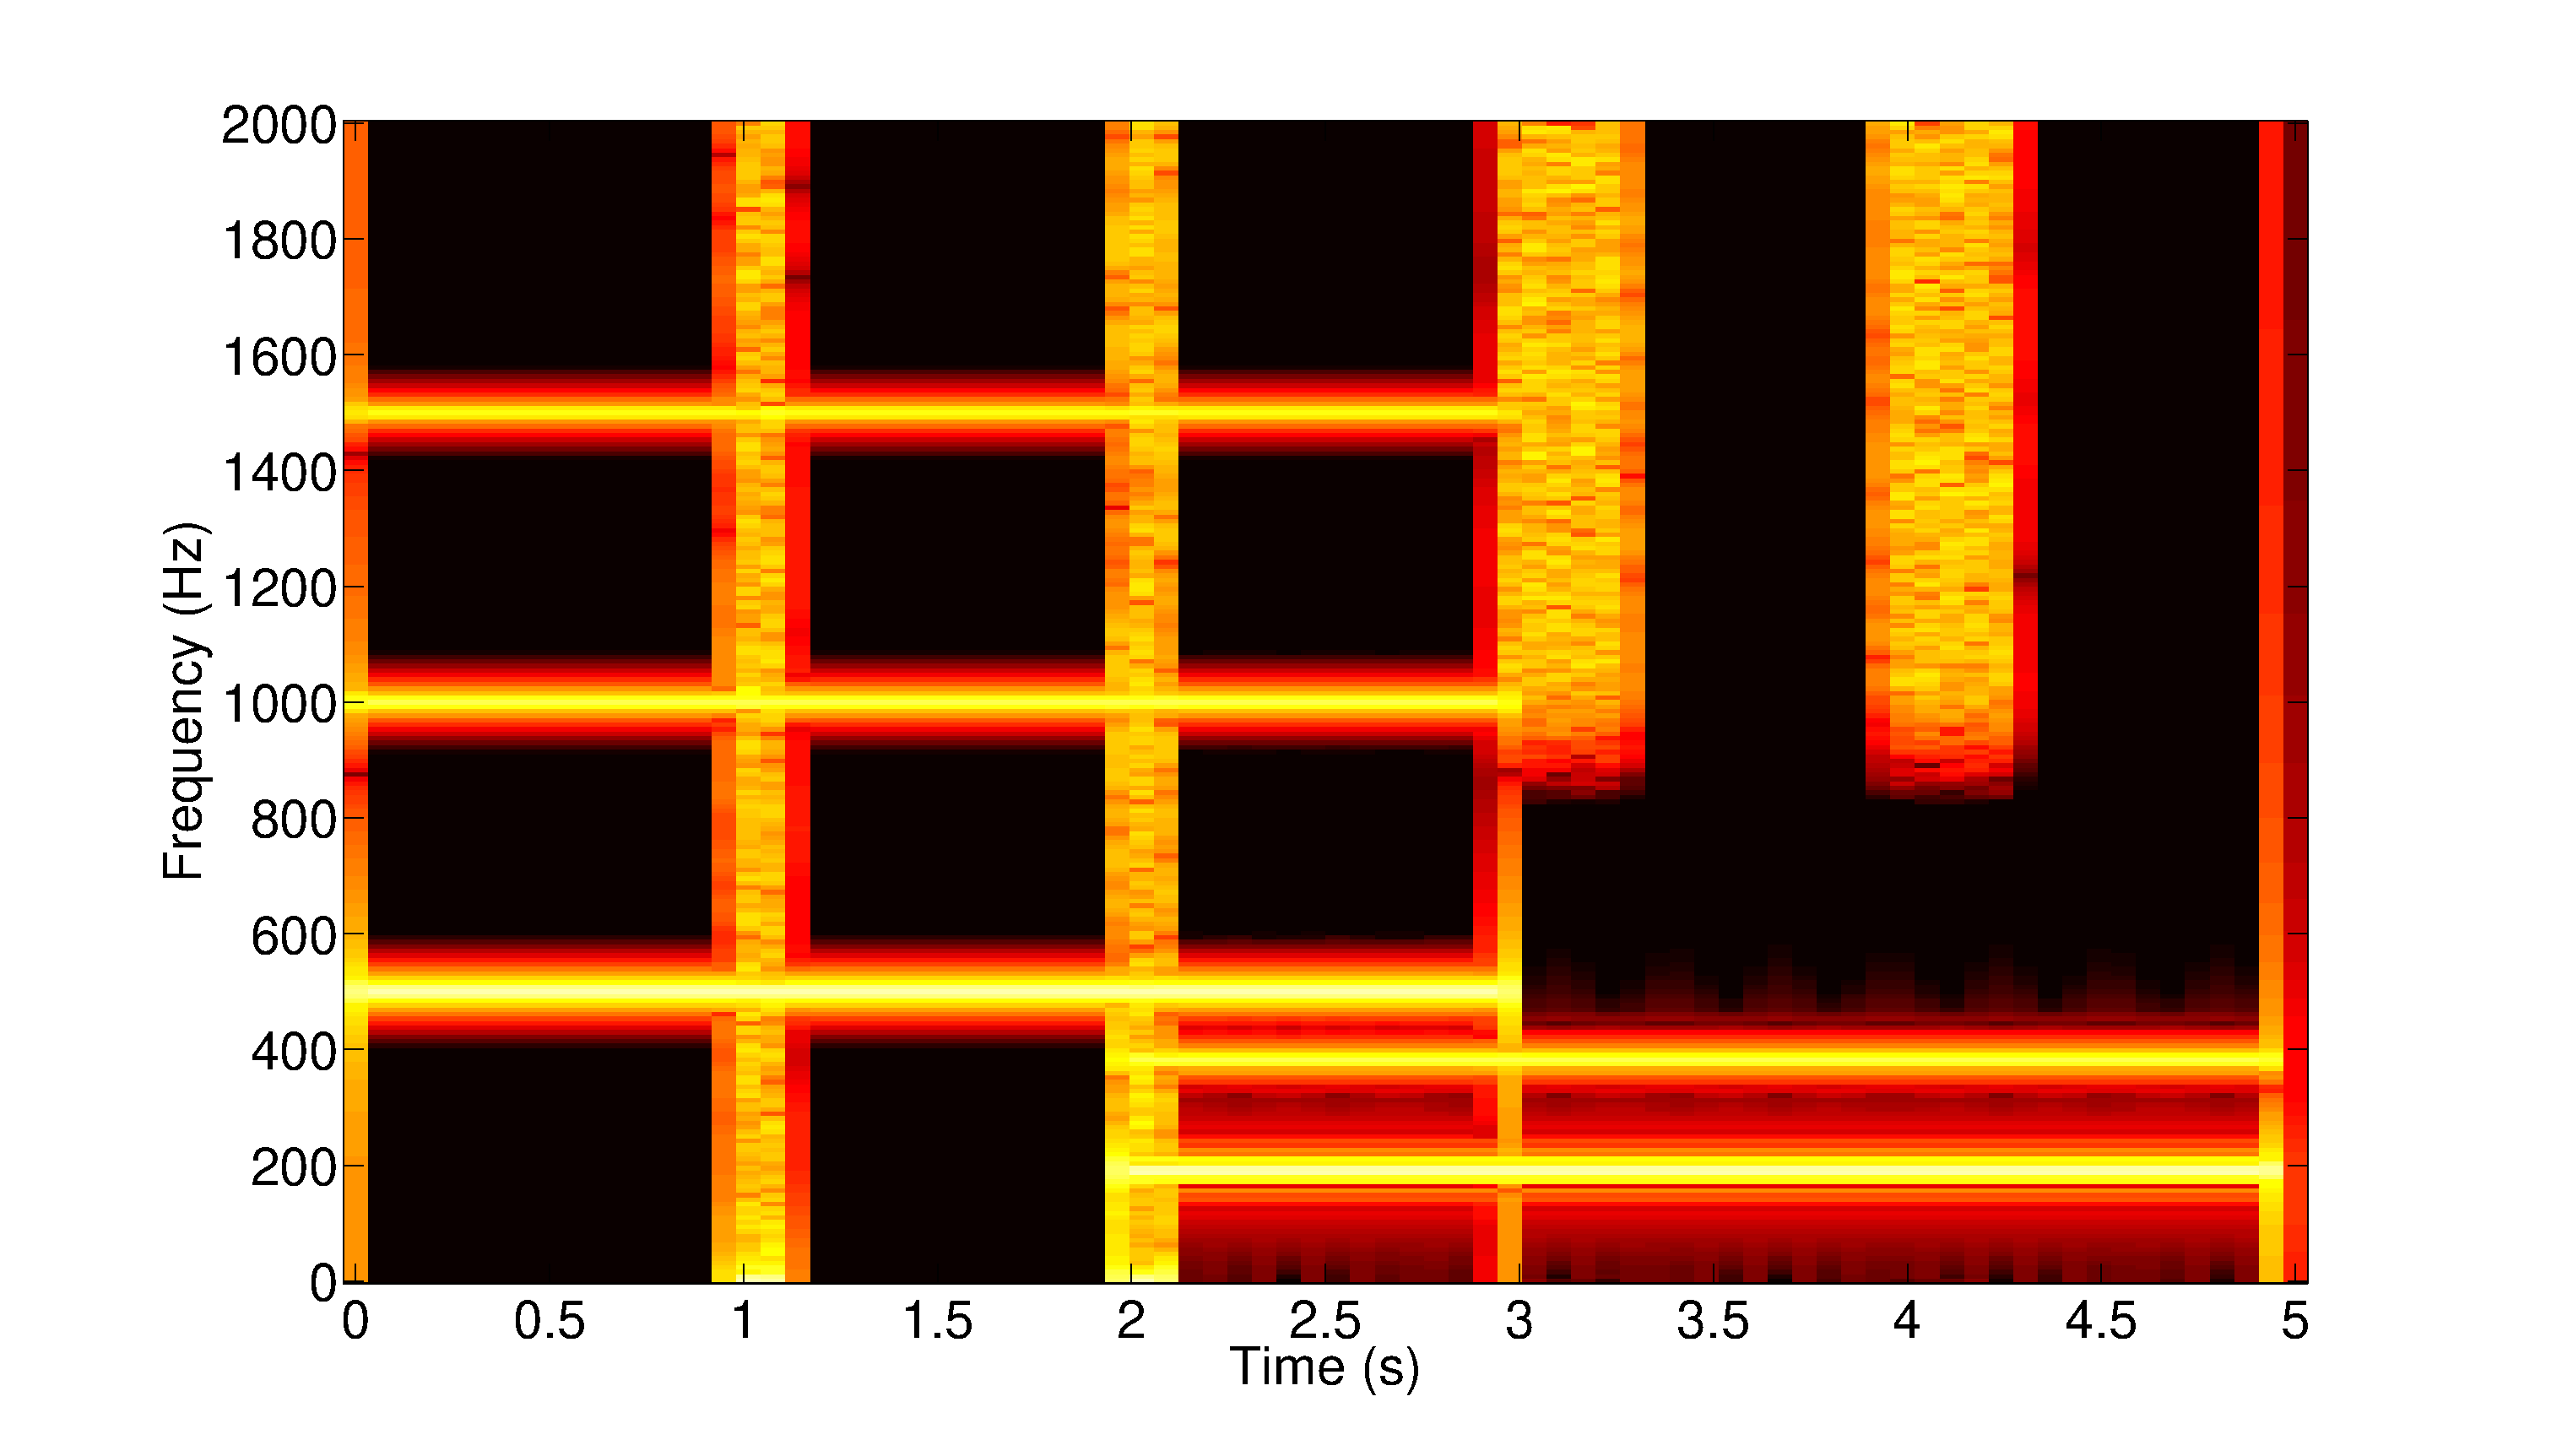
\includegraphics[width=9cm]{fig/synthetictestspectrogram}
%  \vspace{2.0cm}
  \caption{\label{SpectroSynth} Spectrogram of the synthetic test signal.}
  
\end{figure}

\begin{figure*}
   
	\centering    
  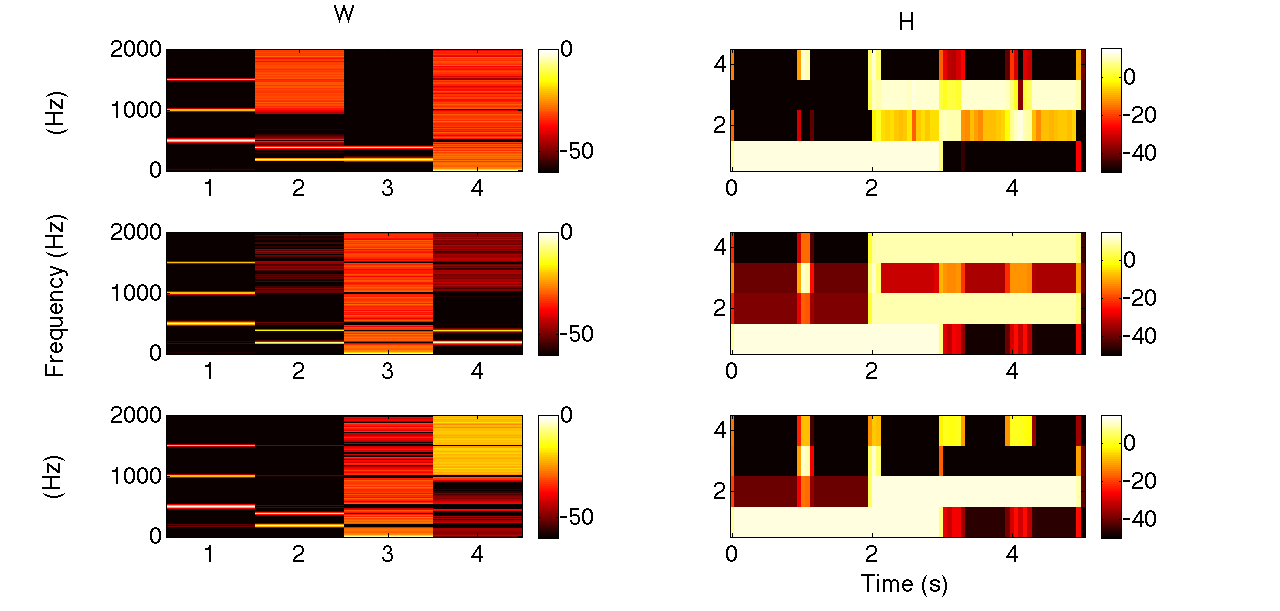
\includegraphics[width=15cm]{fig/WHcomp}

\caption{\label{resultONMF2} Results of the decomposition of the NMF (top matrices), PNMF (middle matrices) and SPNMF (bottom matrices).}


\end{figure*}


\subsection{Protocol and details of the test database}


To study the impact of using learned dictionaries in SPNMF (Algorithm \ref{AlgoDictionary}), we run several tests on the public SiSec database from \cite{SiSec10}. This database is composed of polyphonic real-world music excerpts. Each music signal contains percussive, harmonic instruments and vocals. It consists of four recordings whose durations range from $14$ to $24$~s. Our goal is to perform a harmonic/percussive decomposition. Thus, following~\cite{canadas2014percussive}, we do not consider the vocal part and we build mixture signals only from the percussive and harmonic instruments. All the signals are sampled at $44.1kHz$. We compute the STFT with a $1024$ and $2048$ sample-long Hann window with a $50\%$ overlap.
Three tests are run on these data:
\begin{enumerate}
	\item The first test aims at assessing the robustness of the SPNMF with respect to the rank of the PNMF part. 
	\item The second test is to evaluate which of the three divergences (Euc, KL and IS respectively) give the best harmonic/percussive decomposition results.
	\item The last test shows the influence of the dictionary on the separation performance. 
\end{enumerate} 
Note that the database we use for tuning the proposed method is different from the one in the evaluation phase in order to prevent any possible over-training and therefore to get the most accurate and fair comparison. 
In order to evaluate and compare the results we then compute the common Signal to Distortion Ratio/Signal to Interference Ration/Signal to Artefact Ratio (SDR/SIR/SAR) metrics for blind source separation with the BSS-Eval toolbox~\cite{bsseval}. 



\subsection{Comparison between PNMF and regularized NMF}




\subsection{Robustness wrt the rank of the harmonic part}
\label{setup:rank}

In the case where we use a fixed dictionary matrix, the only parameter of the algorithm is the rank of factorization of the harmonic part. In this experiment, we use the SPNMF algorithm with the fixed dictionary obtained from the STFT of a drum signal as described in Section~\ref{fixedict}. The algorithms are implemented using the multiplicative update rules from~\ref{euclidisteq},~\ref{KLdisteq} and~\ref{ISdisteq} and they all are  initialized with the same random non-negative matrices. 
We display the mean value of the separation results on Figure~\ref{RankOfFact}. When the rank of factorization is small, the Euclidean distance and the KL divergence do not give satisfying results. However, for $r>=100$, the results for both distances remain stable. With the IS divergence, the results seem independent of the rank of the factorization.

The optimization process of SPNMF is straightforward thanks to the robustness of the method wrt the rank of factorization. The number of components that can be decomposed by orthogonal basis functions is limited, and increasing the rank of factorization does not perturb the results as the harmonic part has to be orthogonal. For the rest of the article, the rank of factorization will be set to $r=100$ for all methods.



\begin{figure}[t]

  \centering 
  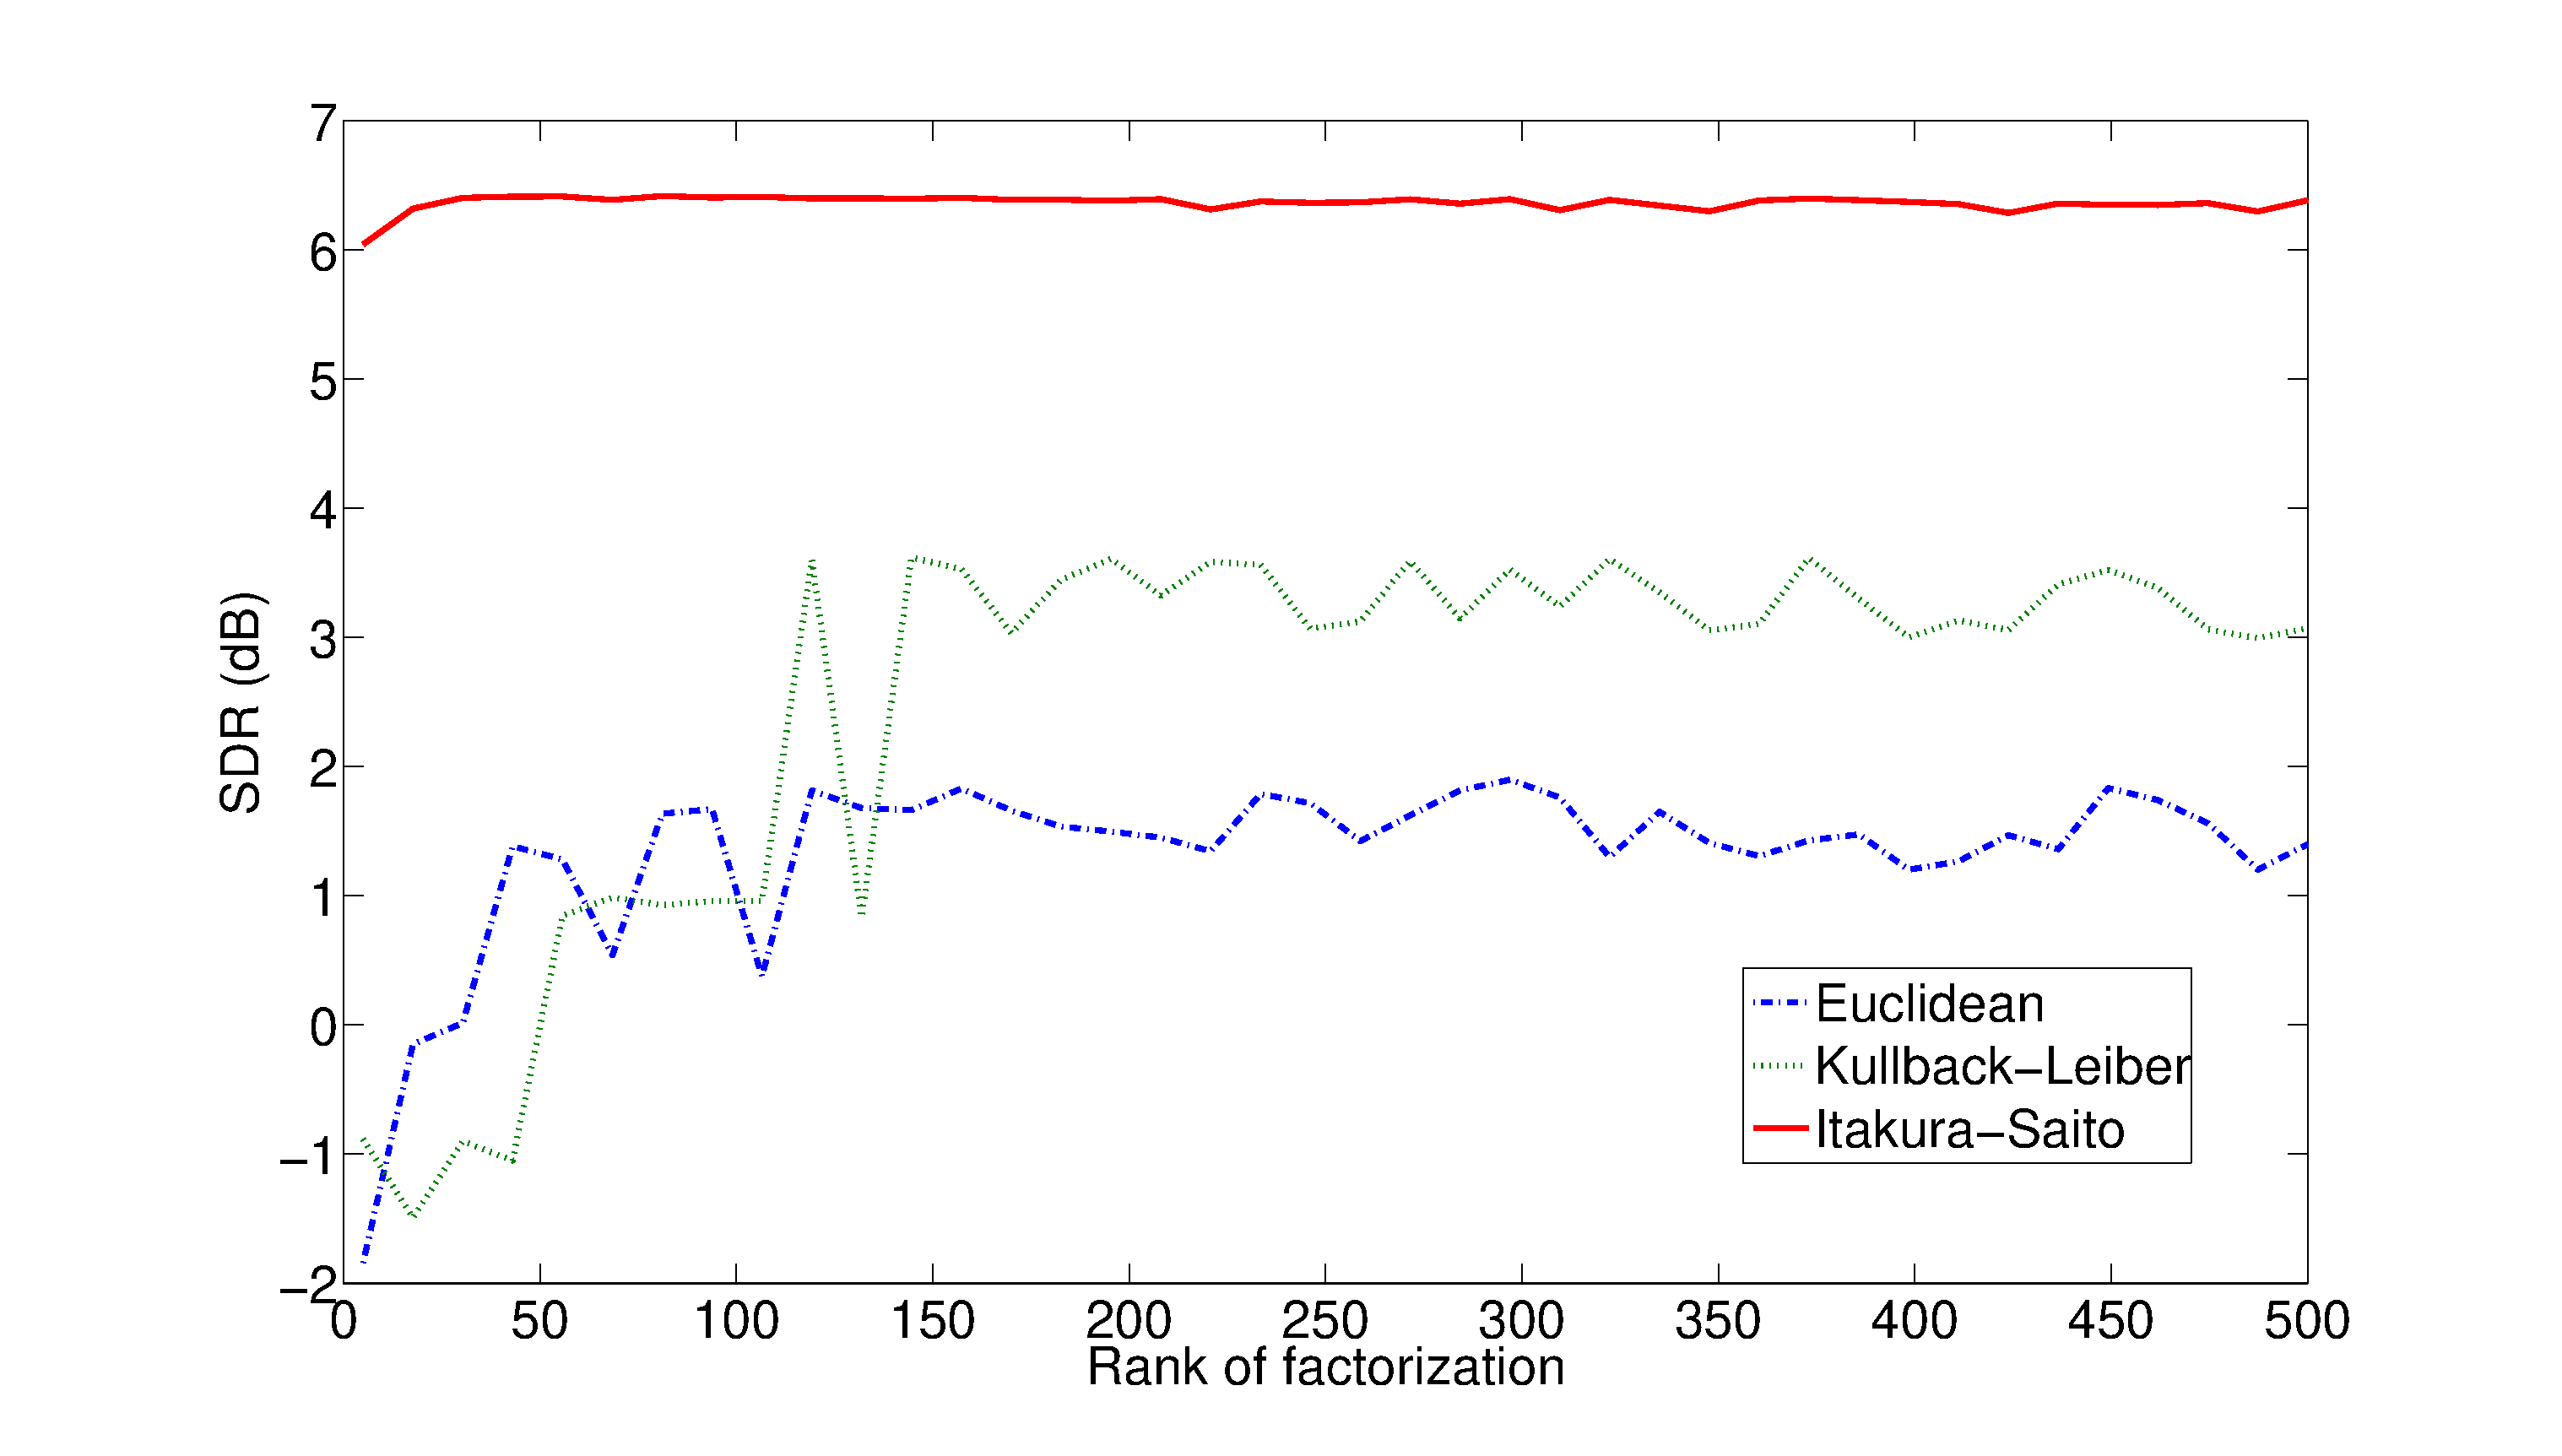
\includegraphics[width=9cm]{fig/RankOfFact}
%  \vspace{2.0cm}
  \caption{\label{RankOfFact} Optimization of the rank of factorization with the three divergences.}
  
\end{figure}




\subsection{Influence of the divergence}
\label{setup:divergence}

In this section we discuss the influence of the divergence in the results of the SPNMF algorithm. It has been established that the IS divergence is well suited for audio signal decomposition~\cite{gray1980distortion}, even if it does not always lead to superior separation performance~\cite{canadas2014percussive}. In this section, we perform a comparison of the three divergences on the SiSec database. Also, we compare two different window lengths ($1024$ samples and $2048$ samples) for the Fourier transform as it showed interesting results. We display on Figures~\ref{frame1024} and~\ref{frame2048} the mean of the results of the three algorithms computed on the SiSec database. Each box-plot is made up of a central line indicating the median of the data, upper and lower box edges indicating the $1^{st}$ and $3^{rd}$ quartiles while the whiskers indicate the minimum and maximum values. 

When the analysis window length is small, the percussive instruments are well represented and the energy is localized. Using a longer window spreads the percussive energy while the tonal components are well separated in the TF domain.

When the window size is small, Figure~\ref{frame1024} shows that the percussive decomposition is better for the Euclidean distance and the KL divergences. However, the harmonic components are not well separated in the TF domain and the orthogonal part of SPNMF does not perform a good separation.  
In the case of a long window, Figure~\ref{frame2048} shows that the IS divergence works better than the other divergences. The orthogonal part is more effective to extract the harmonic components as the finer frequency resolution allows for a better separation in the TF domain. The IS divergence is scale invariant. It means that the low energy components of the spectrogram bear the same relative importance as the higher ones which allows a good extraction of the percussive instruments even if the energy is spread temporally.


For the rest of the article, we will use the SPNMF algorithm with the IS divergence and a window size of 2048 samples for the STFT.


\begin{figure}[t]

  \centering 
  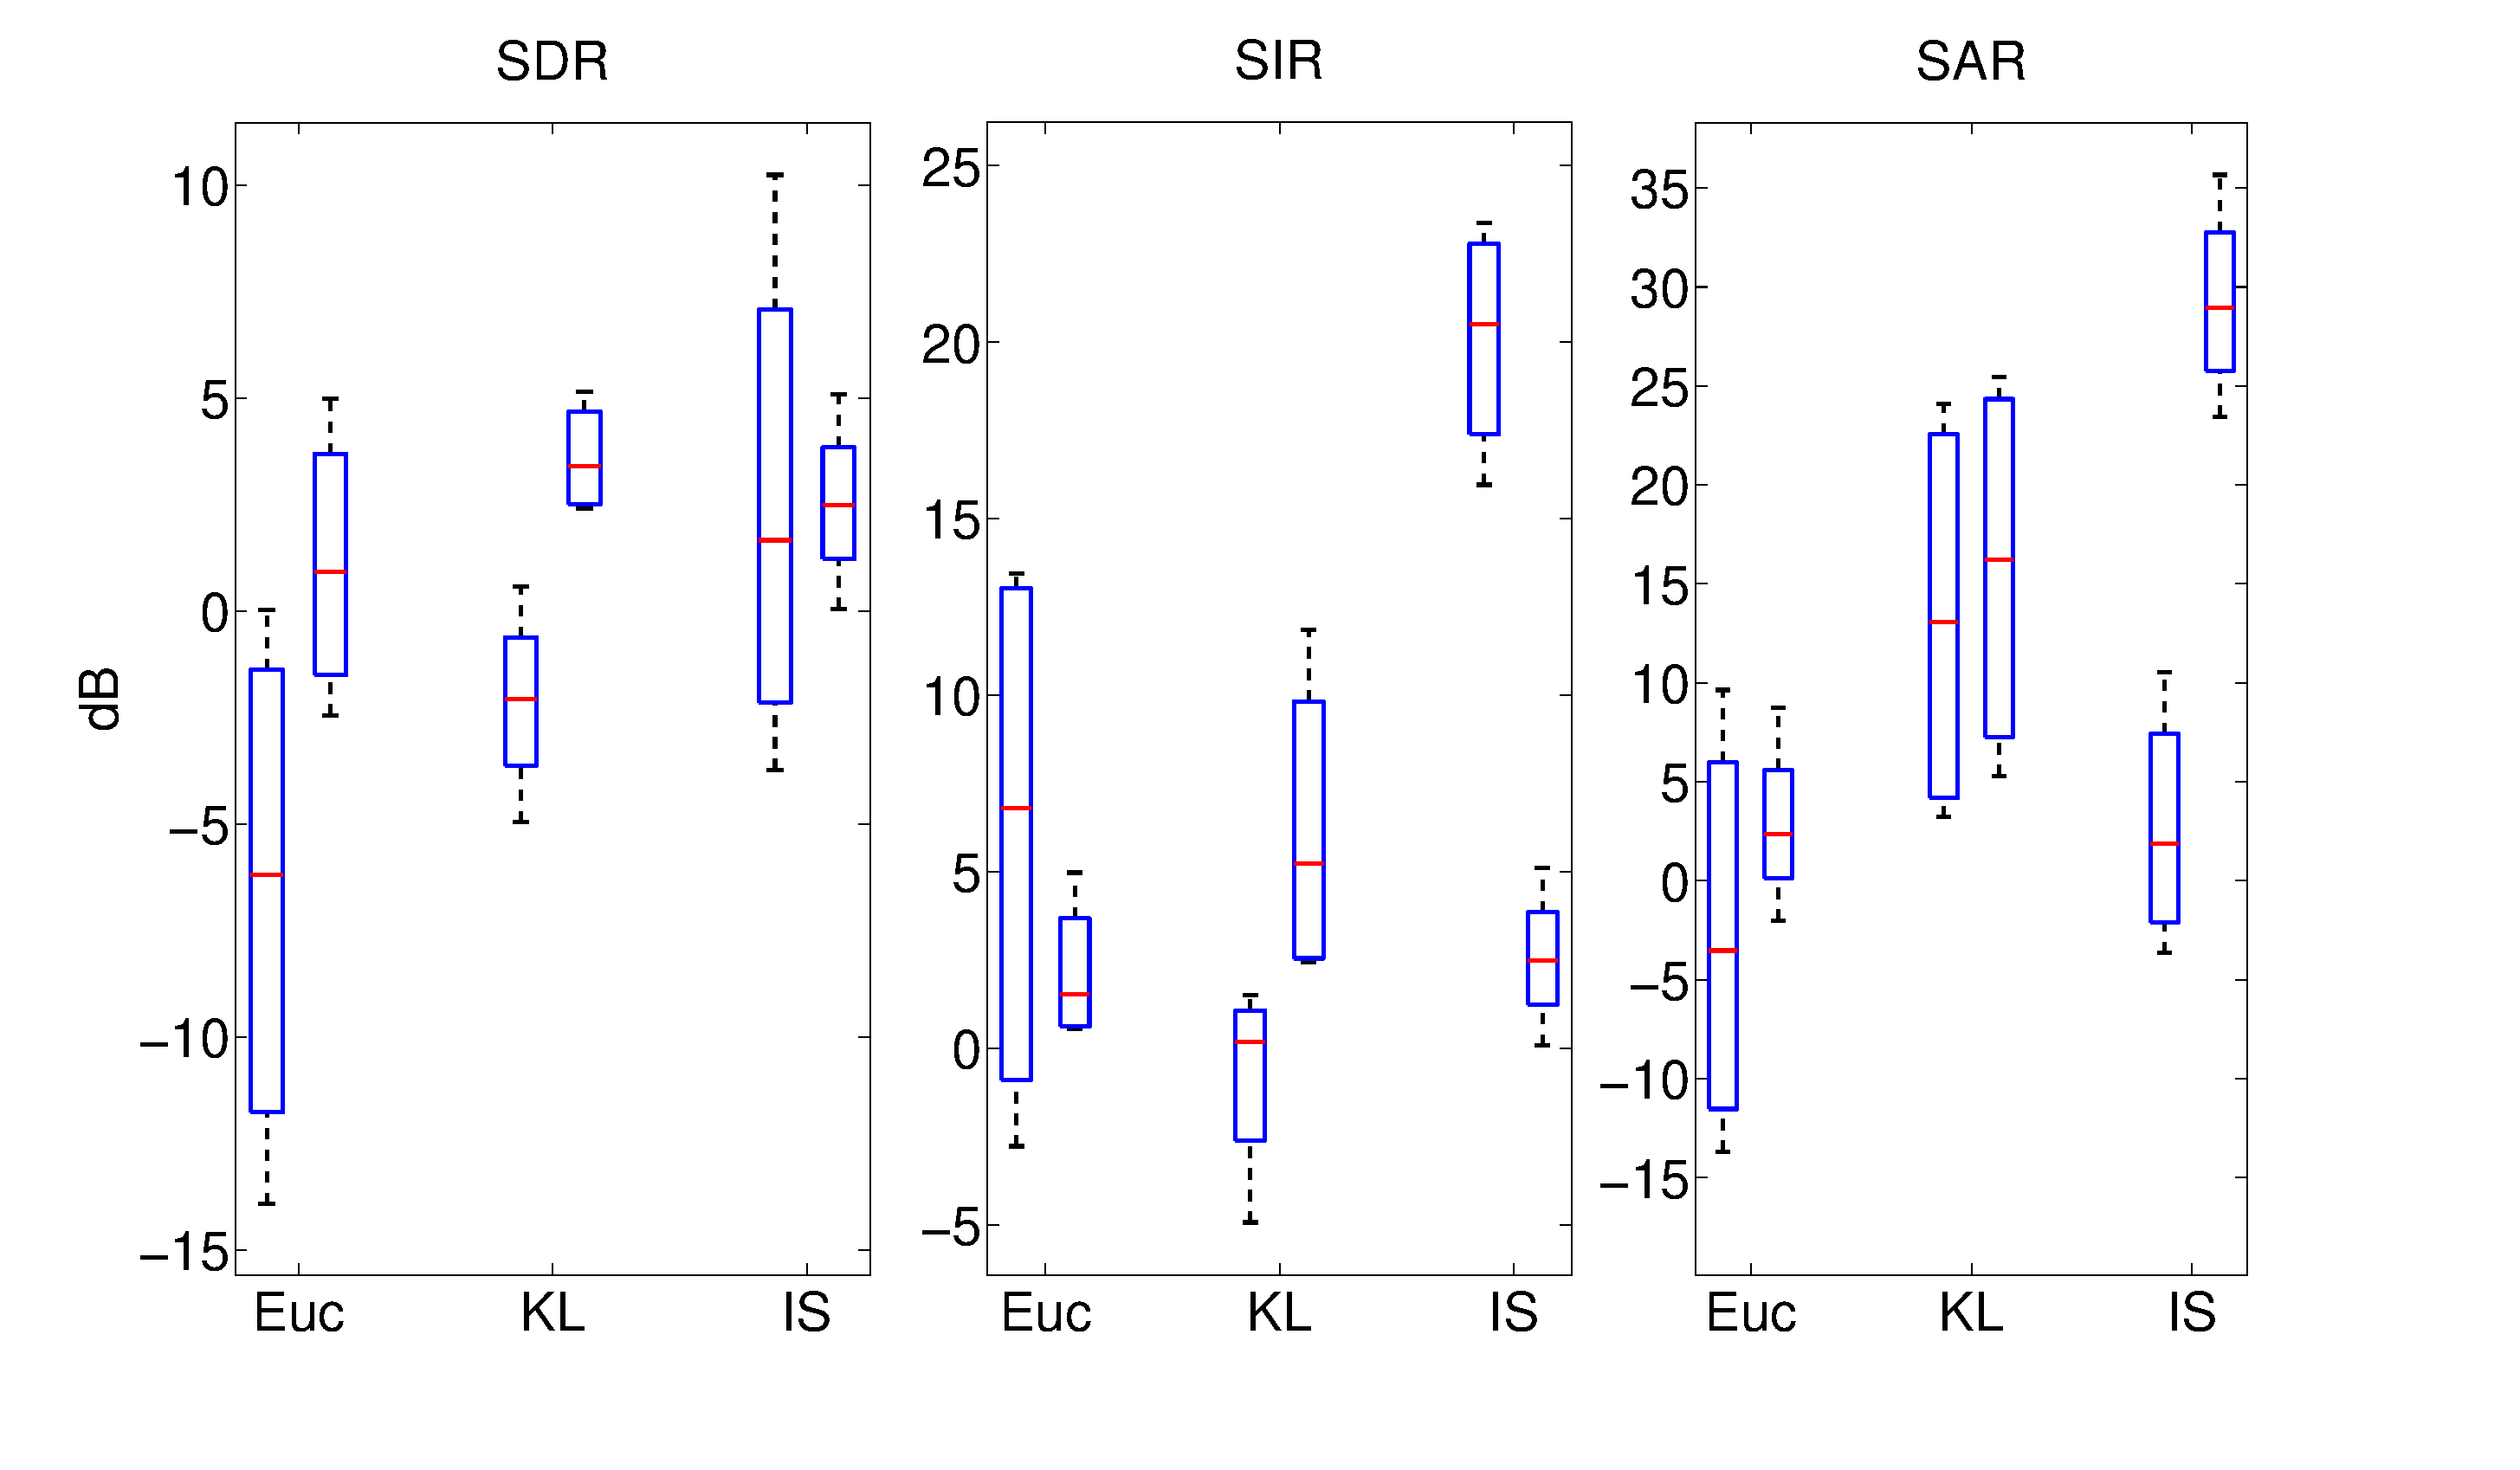
\includegraphics[width=9cm]{fig/NewDictDivTest1024}
%  \vspace{2.0cm}
  \caption{\label{frame1024} SDR, SIR and SAR of harmonic (left bar)/percussive (right bar) estimated sources on the SiSec database with a window frame of $1024$ samples.}
  
\end{figure}


\begin{figure}[t]

  \centering 
  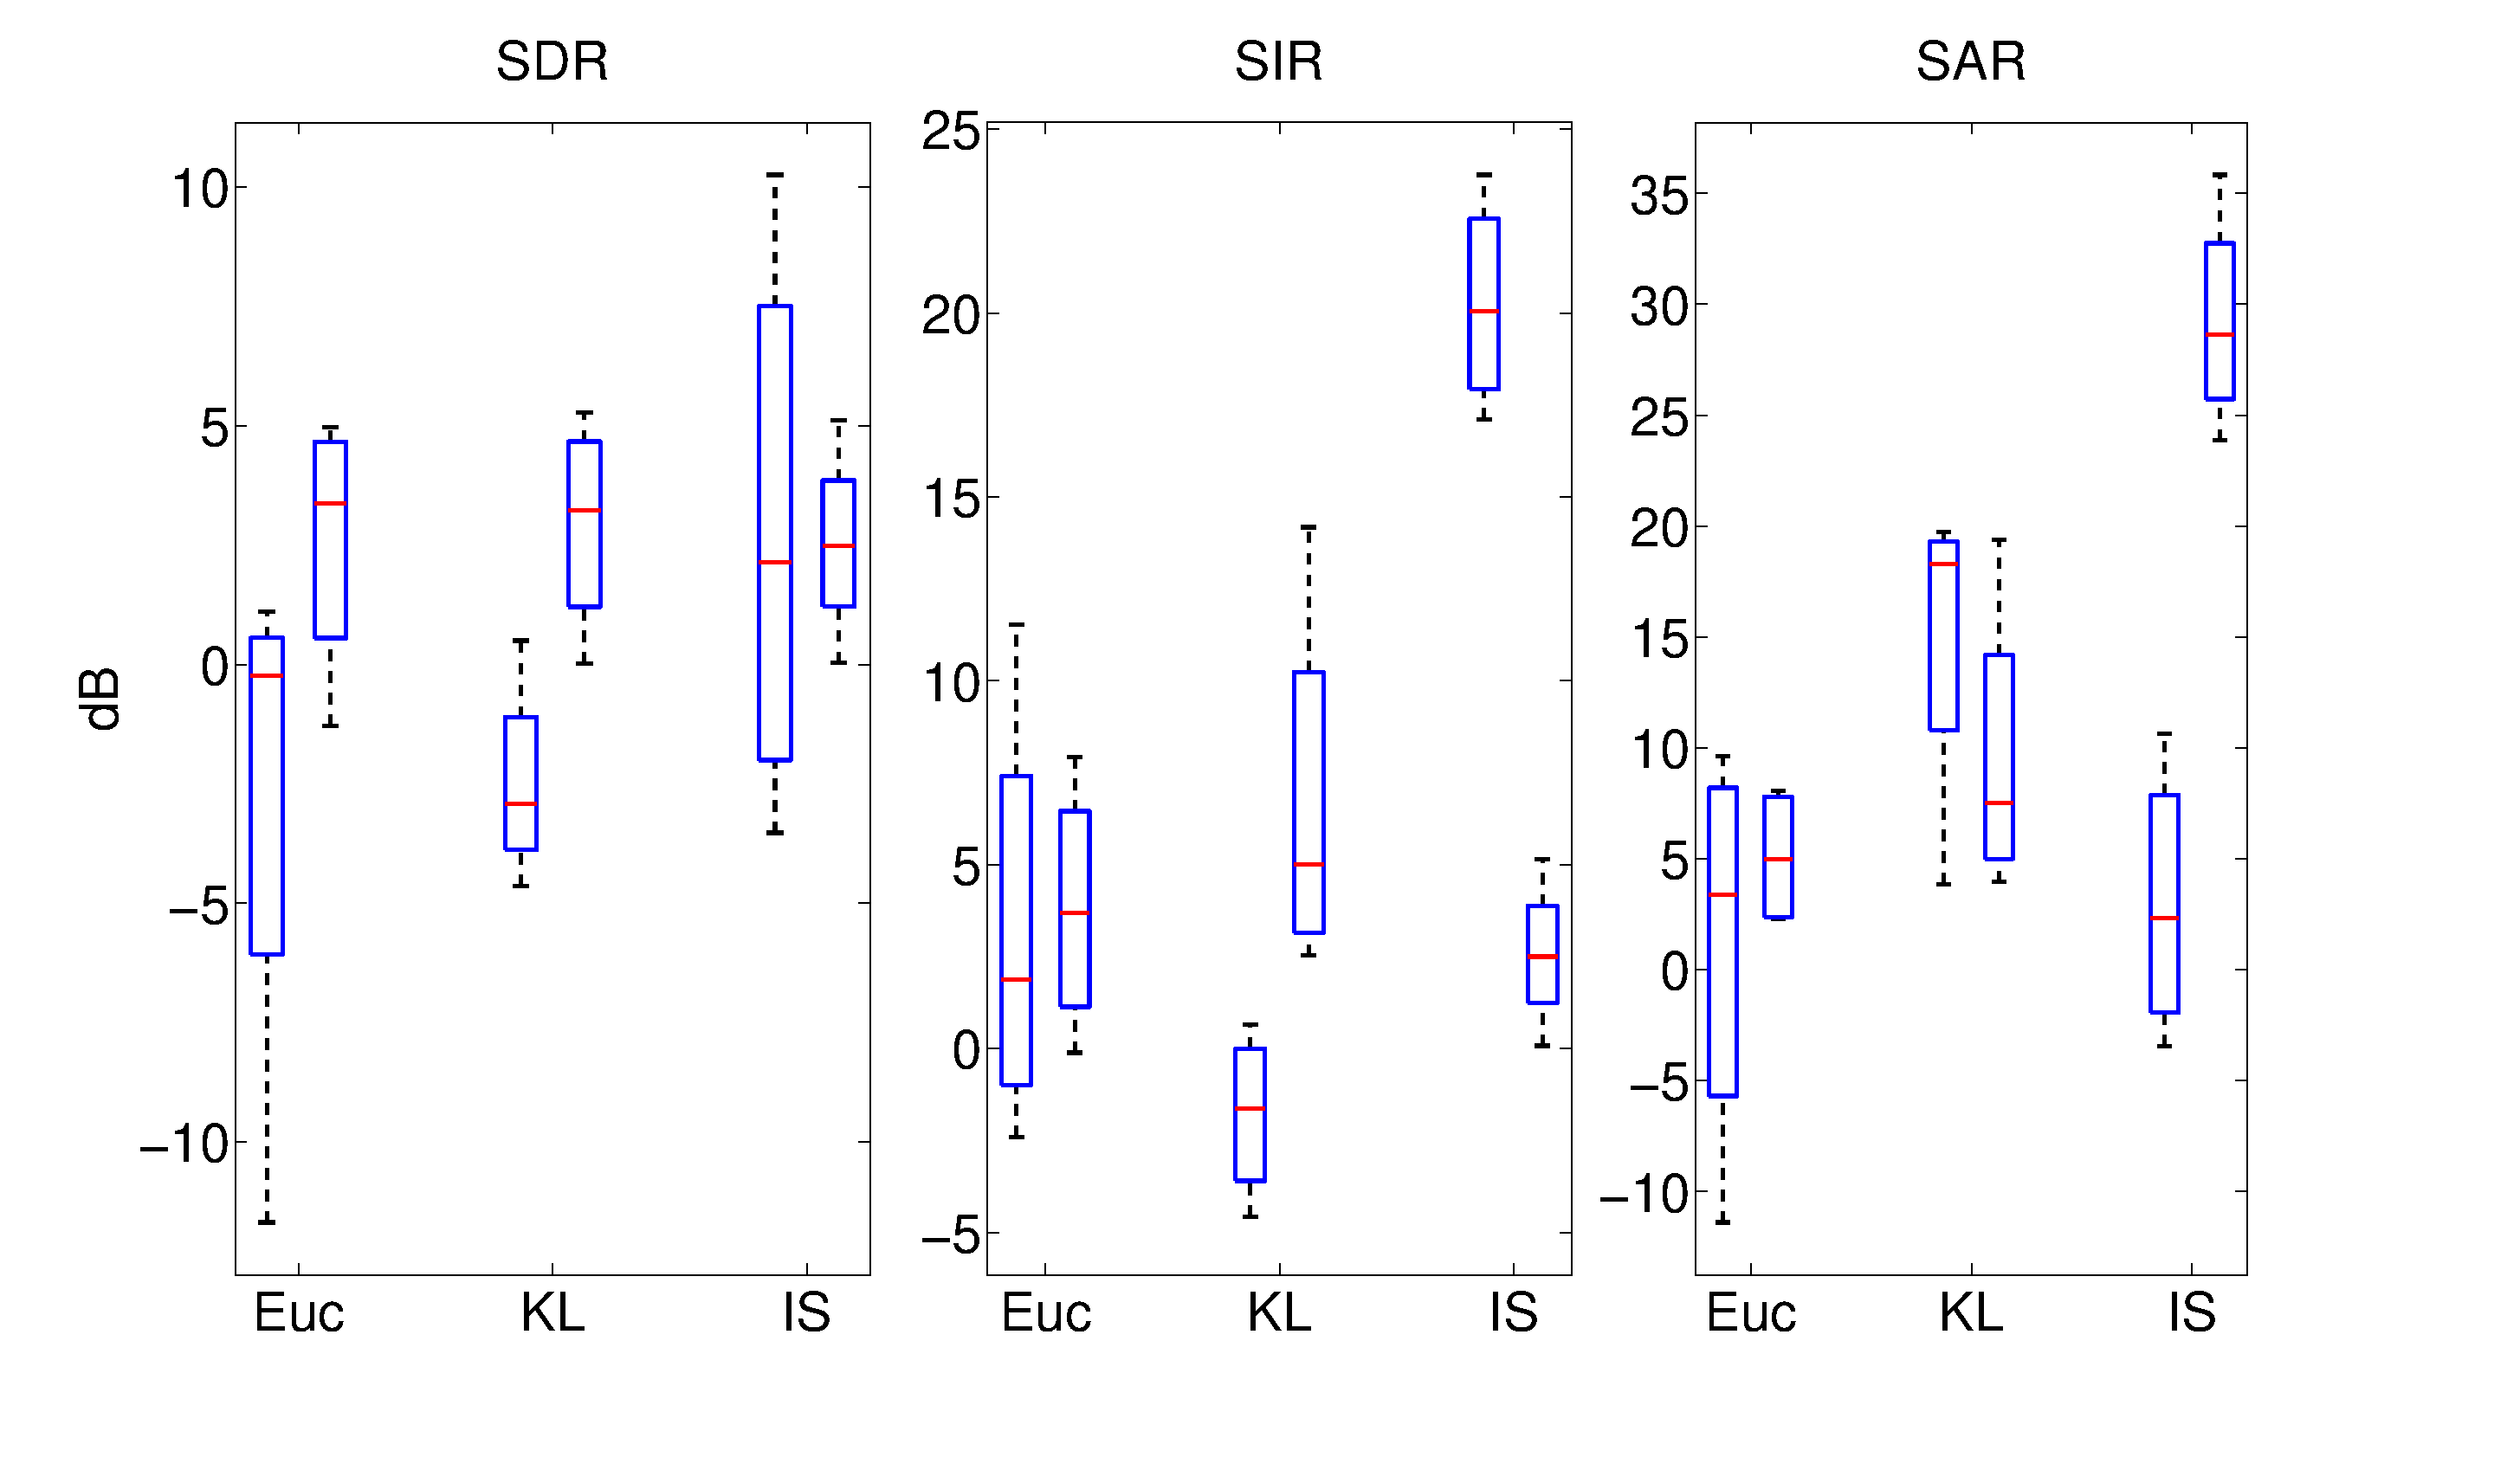
\includegraphics[width=9cm]{fig/NewDictDivTest}
%  \vspace{2.0cm}
  \caption{\label{frame2048} SDR, SIR and SAR of harmonic (left bar)/percussive (right bar) estimated sources on the SiSec database with a window frame of $2048$ samples.}
  
\end{figure}



\subsection{Influence of the dictionary}
\label{setup:dictionary}

%We now discuss the influence of the dictionary. We compare the two methods described in Section~\ref{fixedict}. In addition to that, we test a third dictionary is made by the concatenation of the first two dictionaries. The more information contained in the dictionary, the likely the decomposition to properly extract the percussive part. On some signals, the algorithm is not able to extract a lot of energy from the mixture as no atom from the dictionary correspond to any of the percussive signal.
%We display on Figure~\ref{resultsDict} the SDR results of the decomposition using the NMF dictionary, the STFT dictionary as well as the concatenated dictionary. The SAR and SIR are postponed in Appendix~\ref{appendix:dict} on Figures~\ref{resultsDictSAR} and~\ref{resultsDictSIR} respectively. In our tests, the results with the concatenated dictionary give the highest score. Indeed, the concatenated dictionary contains the largest amount of information and as a result, obtains the best separation. As the dictionary is fixed, it is important to have a large dictionary to be able to extract a large type of percussive instruments. The STFT and the NMF dictionaries give results similar to each other. The two dictionaries contain complementary information that allow for a better separation while they are concatenated. In the tests we will conduct later in Section~\ref{sec:stateoftheart} on a large database, we will use the concatenated dictionary as it contains the largest amount of information. 

We now discuss the different methods to construct the drum dictionary. As the dictionary is fixed, it is important to find a good compromise with the size and the quantity of information contained. 
Two types of audio recordings are available, the first type contains drum hits of the independents element of the drum kit. We concatenated the recording of the drum hits of each drummer in three $10$~min long audio signals. The other type of audio files are drum phrases. We created three signals of different length ($6$~min, $12$~min, $30$~min) for the three drummers for a total of $9$ audio signal. 
Finally, we compute the STFT of these $12$ signals and we execute a NMF on each of the spectrograms to obtain various dictionaries. The rank of the decomposition is chosen as $k \in [6,9,12,25,50,100,200,500]$. In total, $108$ dictionaries are created. 

Multiple tests are run in order to evaluate the influence of each of the parameters for the training step. The drum kit of each drummer are very different and they provide different information for the decomposition. We display on Figure~\ref{resultsDict} the mean SDR, SIR and SAR results of the average results for each drummer. Figure \ref{resultsDict} shows that the information of the drummer $2$ is the most relevant for our test. The drummer $1$ plays on a very small drum kit that does not contains enough information. Finally the drummer $3$ plays uses a large drumset with many elements that are not usually present in most recording and because of that the dictionary is too diverse.

Now the rest of the experiment are conducted using the dictionaries constructed on the audio files from drummer $2$. Figure \ref{resultsDictLength} show the influence of the length of the training data on the results. Above $6$~min of training data, the quality of the decomposition decreases so in the rest of the experiment, we used the dictionaries computed of these data.

Finally, Figure \ref{resultsDictD2} show the results wrt the rank of factorization. The best results are obtained for $k=12$. Bellow that, the dictionary is too small and not enough information is captured. Inversely, if the rank is chosen too big during the learning process, the dictionary does not capture the percussive part satisfyingly during the decomposition.

For the rest of the article, we will use a dictionary constructed using a $6$~min long audio signal from the drummer $2$ with $k=12$.

\begin{figure}[t]

  \centering 
  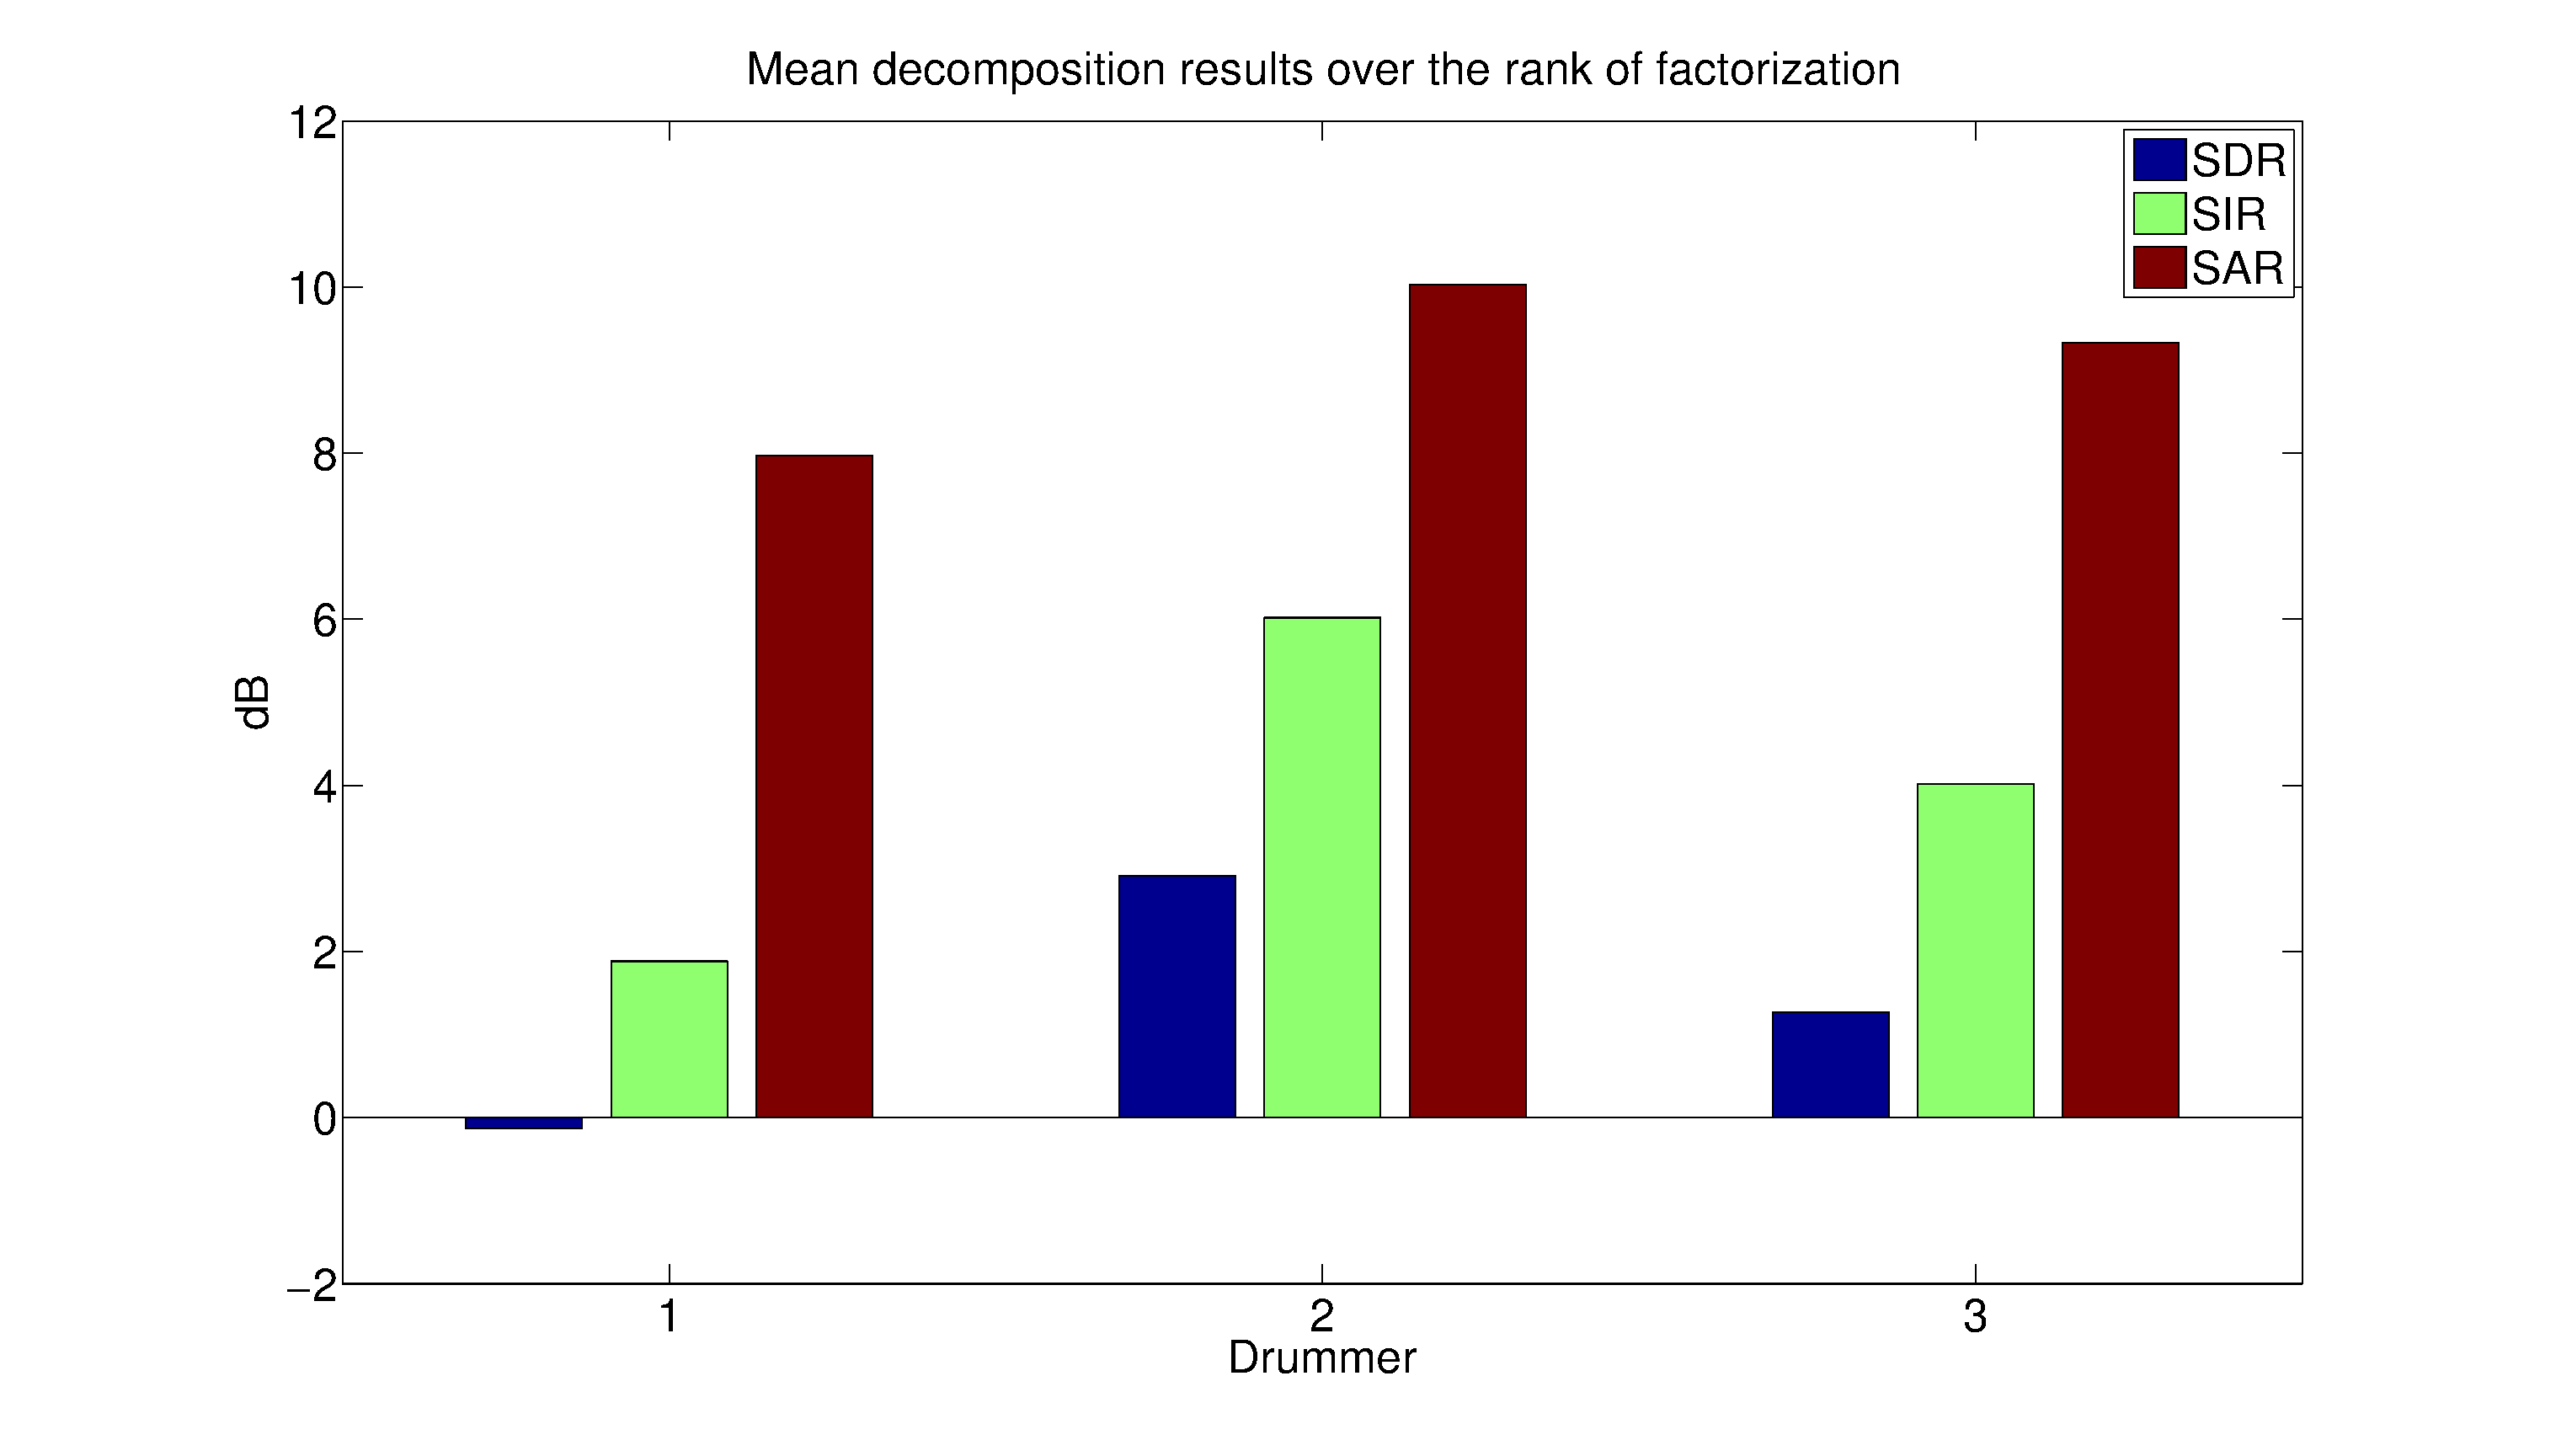
\includegraphics[width=8cm]{fig/ResultsMeanRank}
%  \vspace{2.0cm}
  \caption{\label{resultsDict} Mean SDR SIR and SAR results averaged for each drummer on the SiSec database.}
  
\end{figure}

\begin{figure}[t]

  \centering 
  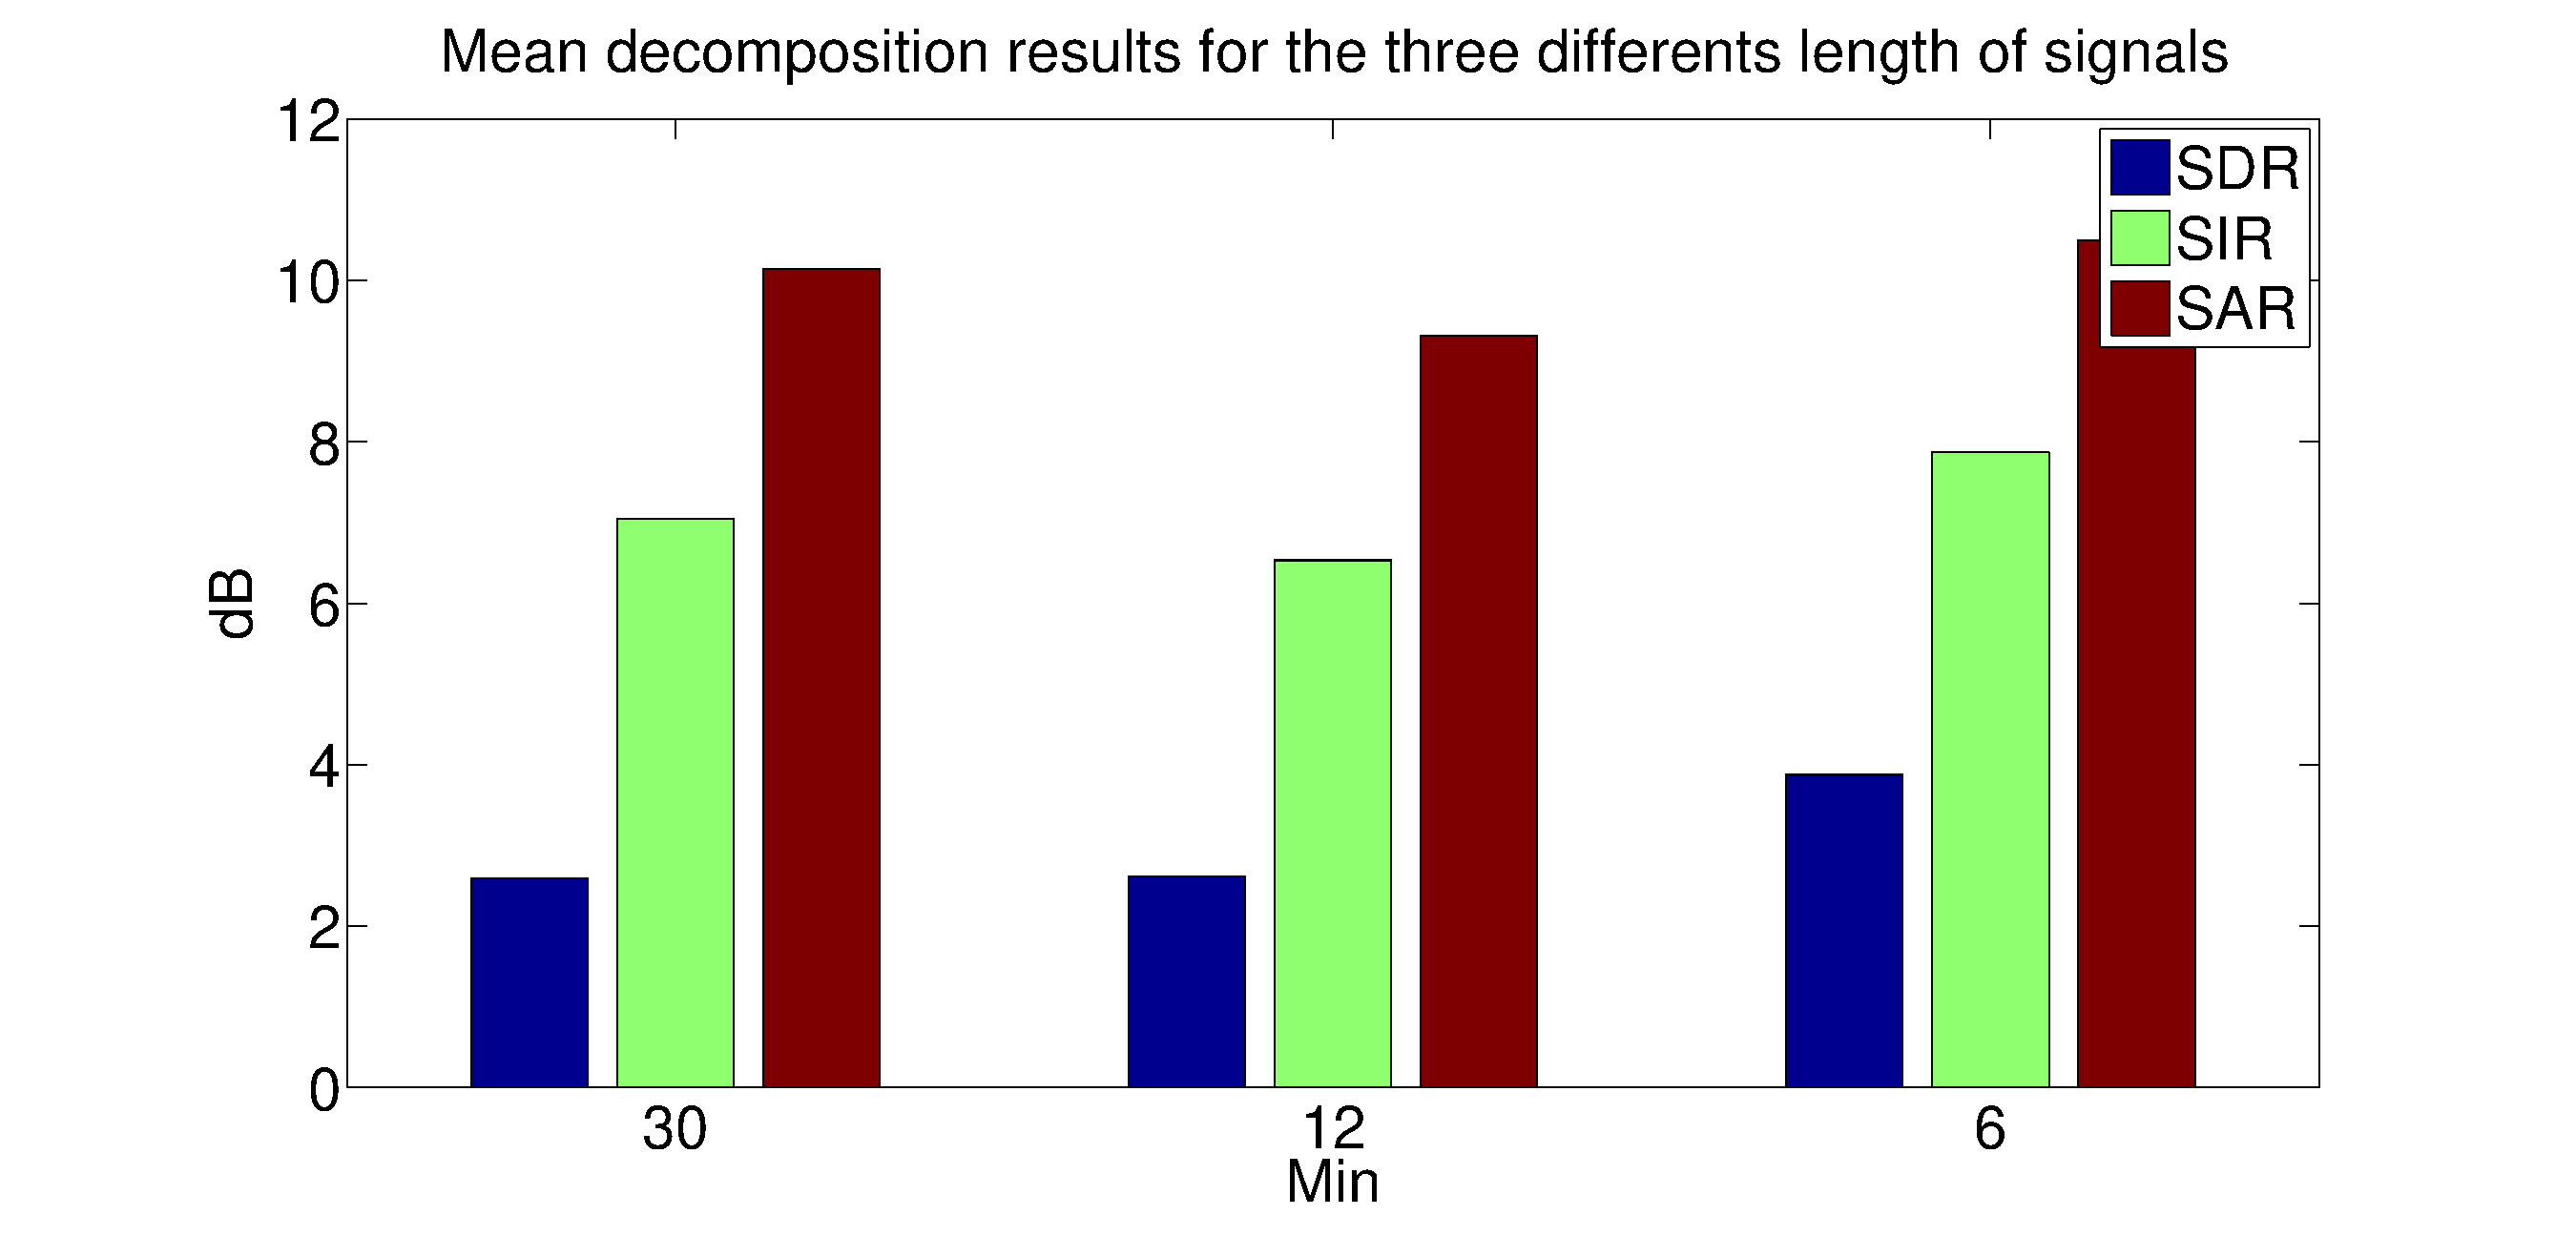
\includegraphics[width=8cm]{fig/ResultsMeanLength}
%  \vspace{2.0cm}
  \caption{\label{resultsDictLength} Mean SDR SIR and SAR results for the dictionaries learned with different signal length on the SiSec database.}
  
\end{figure}
\begin{figure}[t]

  \centering 
  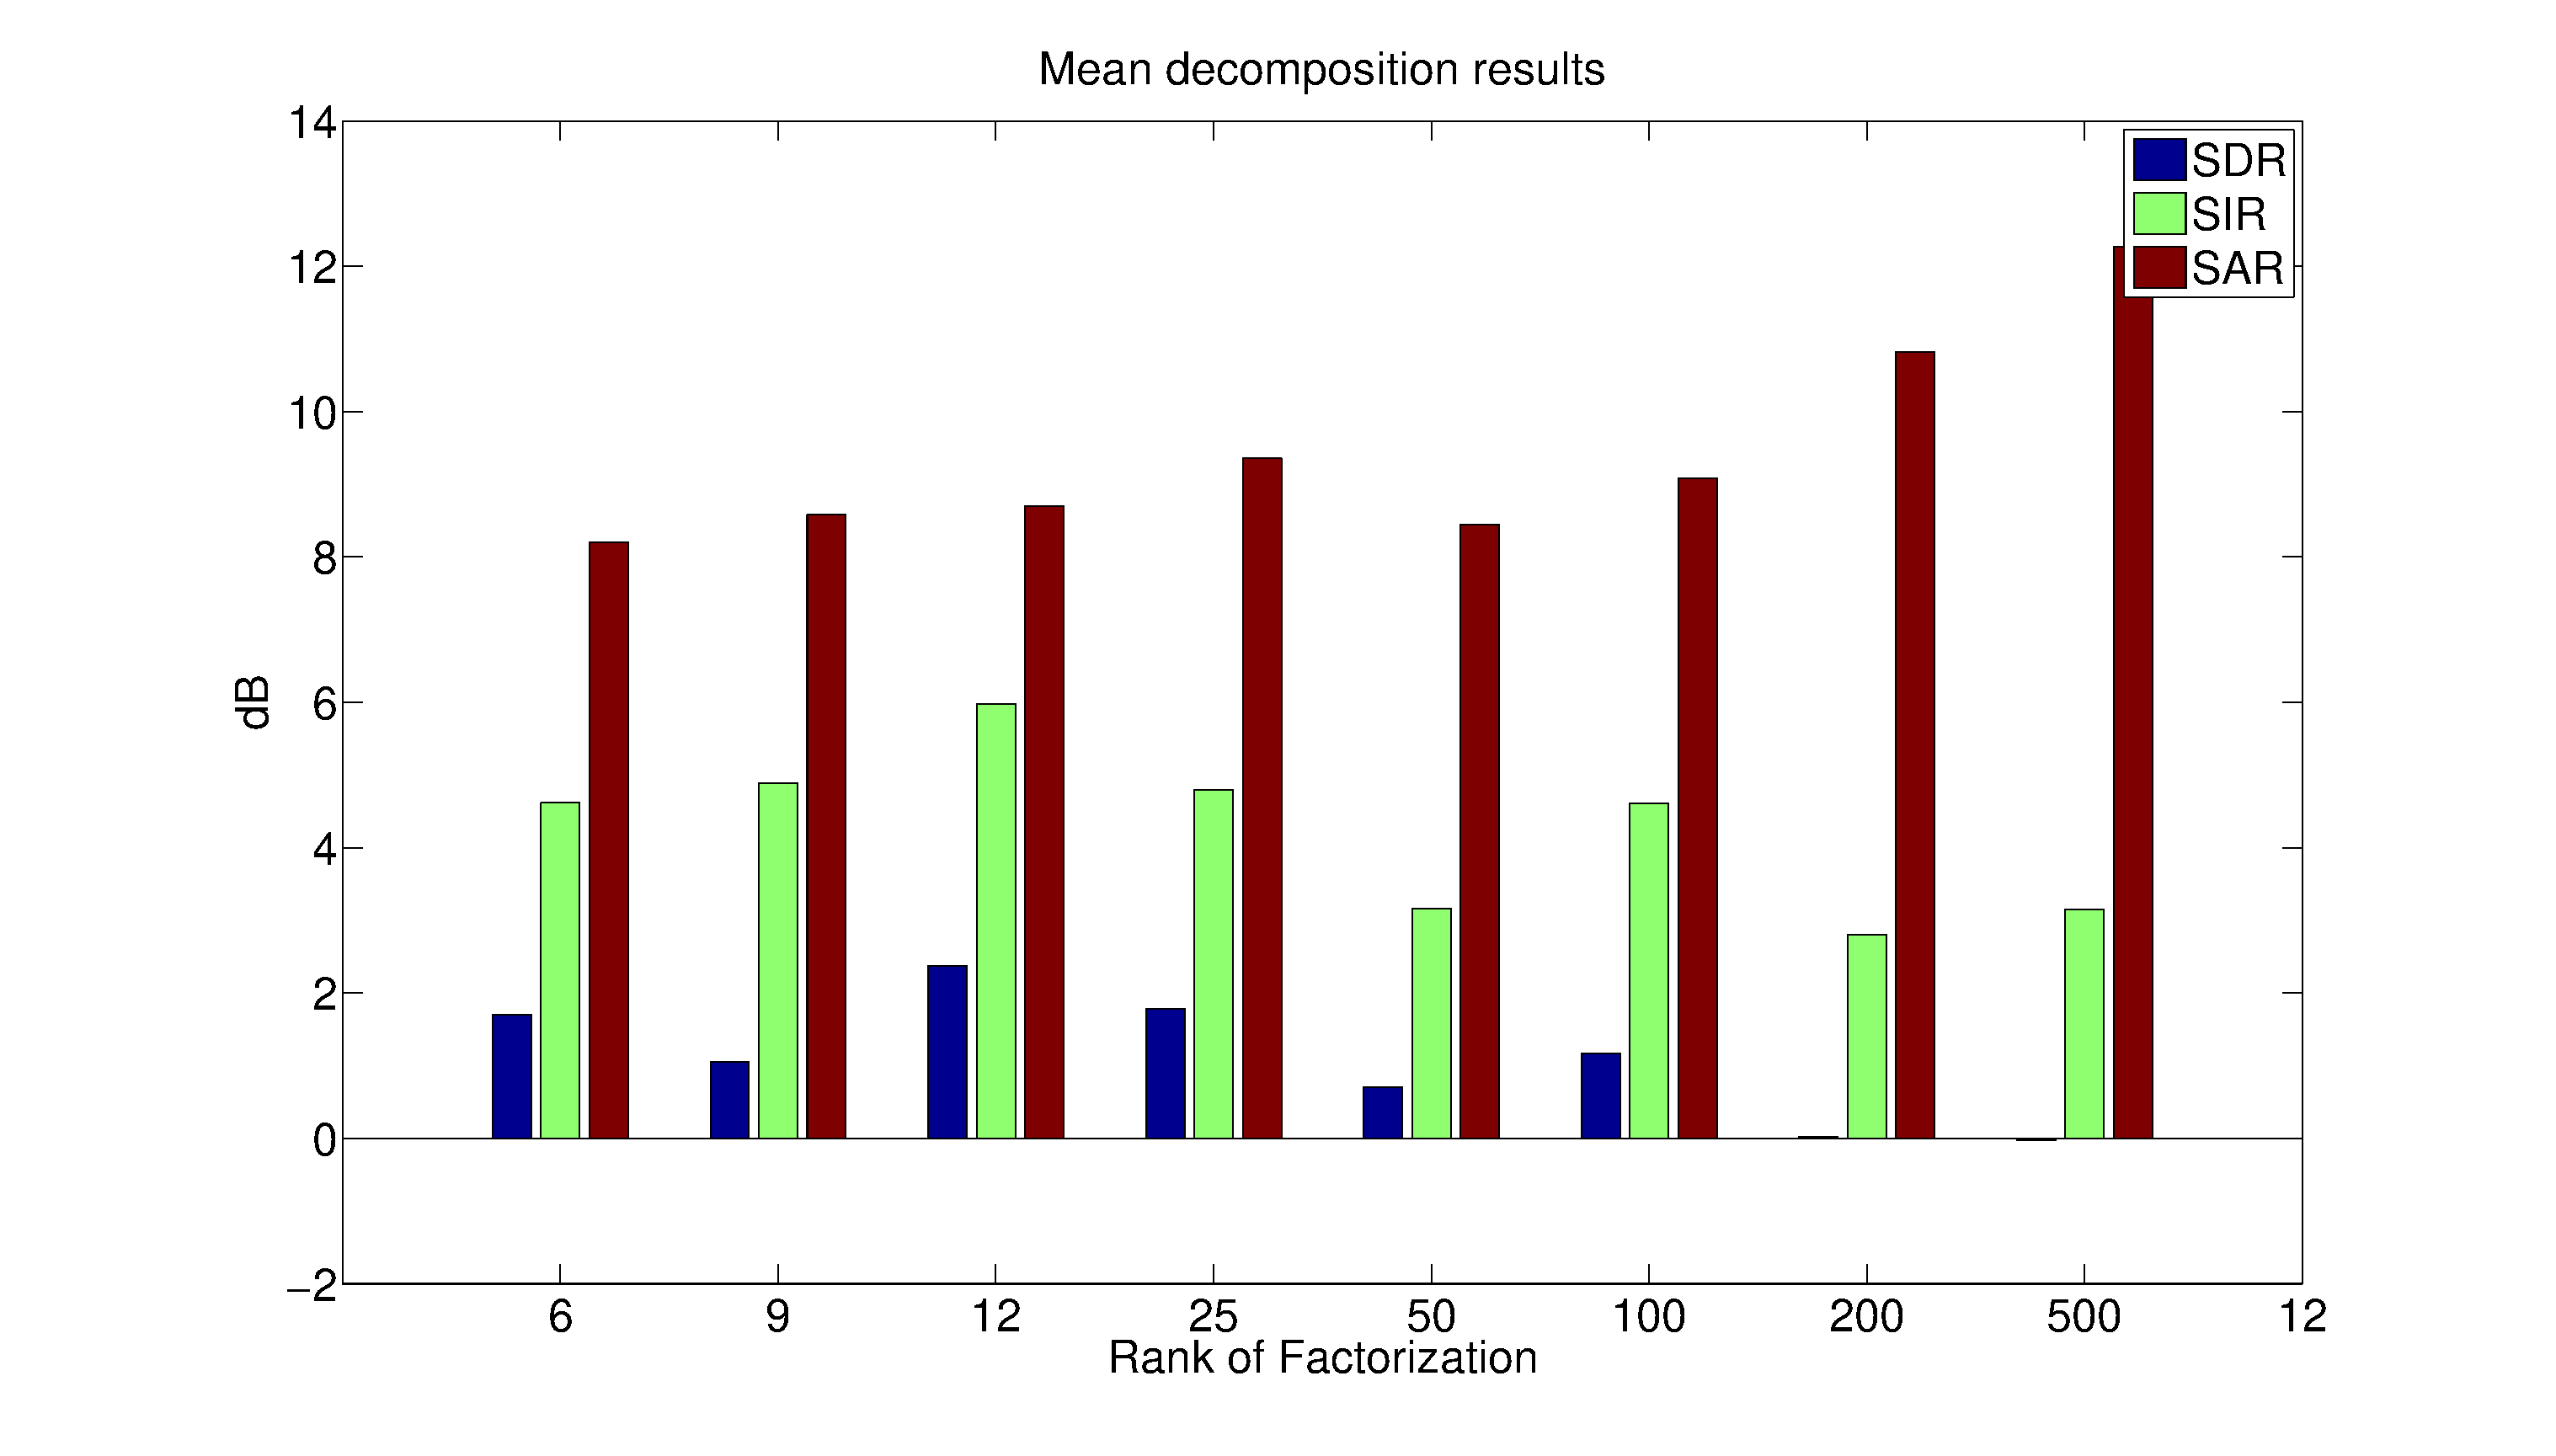
\includegraphics[width=8cm]{fig/ResultsDictDrummer2}
%  \vspace{2.0cm}
  \caption{\label{resultsDictD2} Mean SDR SIR and SAR results for various rank of factorization on the SiSec database.}
  
\end{figure}



\section{State of the art Benchmark}
\label{sec:stateoftheart}

In this section, we compare the proposed method with three state of the art methods on a large evaluation database. We first detail the database used for evaluation and describe the state of the art methods used for comparison in Section~\ref{database} and~\ref{soth} respectively.  


\subsection{Database}
\label{database}

For evaluation, we use the Medley-dB~\cite{bittner2014medleydb} database that is composed of polyphonic real-world music excerpts. It has $122$ music signals and $89$ of them contain percussive instruments, harmonic instruments and vocals. In our tests, the signals that do not contain a percussive part are excluded from evaluation. Because our goal is to perform a harmonic/percussive decomposition, the vocal part is omitted, as in~\cite{canadas2014percussive}. All the signals are sampled at $44.1kHz$.

\subsection{State of the art methods}
\label{soth}

We compare here the SPNMF with the fixed dictionary matrix to three other recent state of the art methods: constrained NMF (CoNMF)~\cite{canadas2014percussive}, HPSS~\cite{fitzgerald2010harmonic} and NMPCF~\cite{kim2011nonnegative}. Constrained NMF and NMPCF are re-implemented in this paper and the HPSS implementation is taken from~\cite{DriedgerMueller14_TSMToolbox_DAFX}.

HPSS is a state of the art, versatile and computationally efficient method. It is widely used in the Music Information Retrieval community and is a good baseline for comparison. The constrained NMF algorithm is the most recent method for harmonic/percussive separation. It gives good results on a small scale test, however the robustness of the algorithm has not been tested yet in a large scale experiment. Finally the NMPCF, similarly to our method, uses a drum dictionary to guide the percussive estimation but the harmonic part is totally unconstrained. 


\subsection{Results} 
\label{subResults}

Figures~\ref{DatabaseSDR},~\ref{DatabaseSIR} and~\ref{DatabaseSAR} show the SDR, SIR and SAR results of the four methods on the selected $89$ songs of the original Medley-dB database~\cite{bittner2014medleydb}. The results on the entire database show that all four methods extract the harmonic instruments much better than the percussive instruments. Our explanation is that all methods rely on Wiener filtering for phase reconstruction (see Equation~\eqref{percuwiener}). As the percussive instruments have flat spectra, the percussive mask is a non sparse matrix and small estimation errors drastically decrease the results of the percussive instruments. This tendency is not visible on small scale tests (see Figure~\ref{resultsDict}). 

Figure~\ref{DatabaseSDR} shows that SPNMF obtains on average the highest separation score for the percussive, harmonic and mean SDR. However, the variance of the results of SPNMF is higher than for the other algorithms. Some songs of the database contain percussive instruments that are not present in the learning database ENST-Drums, such as the tambourine, the bongo, the gong and electronic drums. Because the dictionary is fixed, these percussive instruments are not correctly decomposed by the SPNMF. Some songs are well separated while other obtain much lower results since the percussive part is not well decomposed. This induces an increase of the variance of the results. 

The NMPCF, also based on trained data, is more robust than the SPNMF because the dictionary that extract the drums is not fixed. It allows more freedom and the results are more consistent even if some percussive instruments are not in the learning database. However, the mean score is lower than in the case of the SPNMF.

The HPSS results obtained in our tests are unsatisfying. A wide variety of harmonic instruments in the database have really strong transients and rich harmonic spectra (distorted electric guitar, glockenspiel\ldots). Similarly, some percussive instruments have sparse basis functions localized in the low frequency range (bass drum, bongo, toms\ldots). Because of that, HPSS fails to extract these instruments in the appropriate harmonic/percussive parts. On average, it is able to correctly separate the percussive part (with relatively high SDR and the highest SIR), but it shows a very low SAR compared to the other methods. Similar outcomes have been observed in~\cite{canadas2014percussive} for HPSS.

The constrained NMF algorithm relies on the same hypothesis than HPSS and the results are lower than those of SPNMF. Some transients of the harmonic instruments are decomposed in the percussive part, and some percussive instruments (mainly in the low frequency range) are decomposed in the harmonic part. The method is still competitive in the large scale test. 

%Compared to the other state of the art methods, the SPNMF obtains the higher average results on the selected database. 


\begin{figure}[h]

  \centering 
  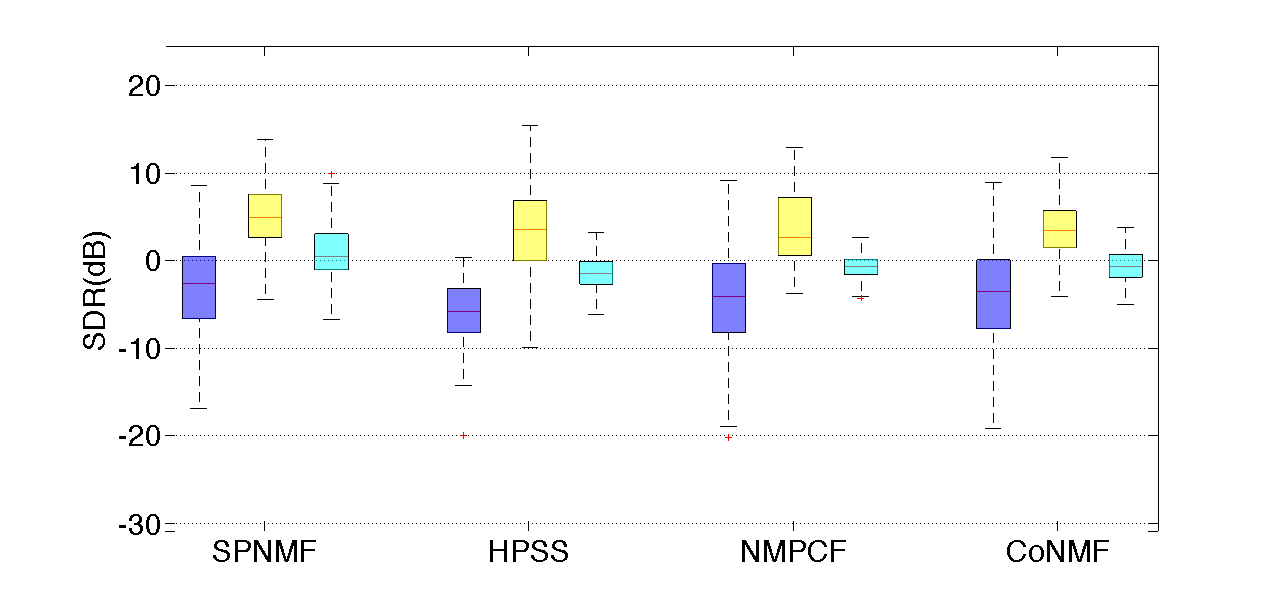
\includegraphics[width=9cm]{fig/DatabaseSDR.eps}
%  \vspace{2.0cm}
  \caption{\label{DatabaseSDR} SDR for percussive/left, harmonic/middle, mean/right separation results on the database for the four methods.}
  
\end{figure}

\begin{figure}[h]

  \centering 
  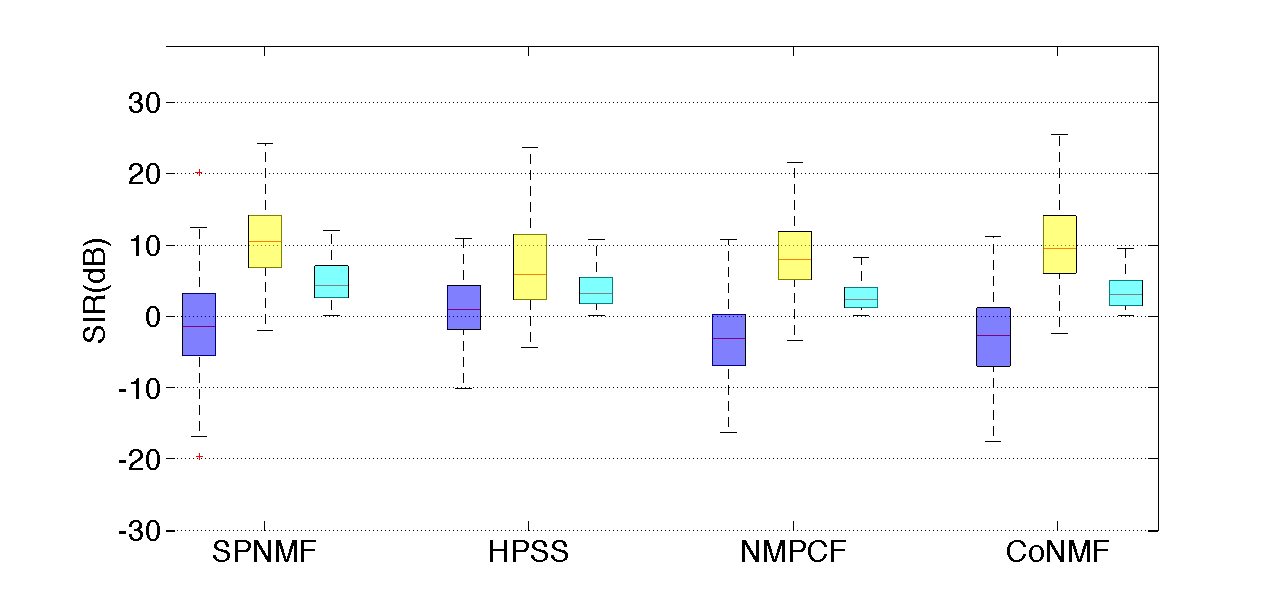
\includegraphics[width=9cm]{fig/DatabaseSIR.eps}
%  \vspace{2.0cm}
  \caption{\label{DatabaseSIR} SIR for percussive/left, harmonic/middle, mean/right separation results on the database for the four methods.}
  
\end{figure}

\begin{figure}[h]

  \centering 
  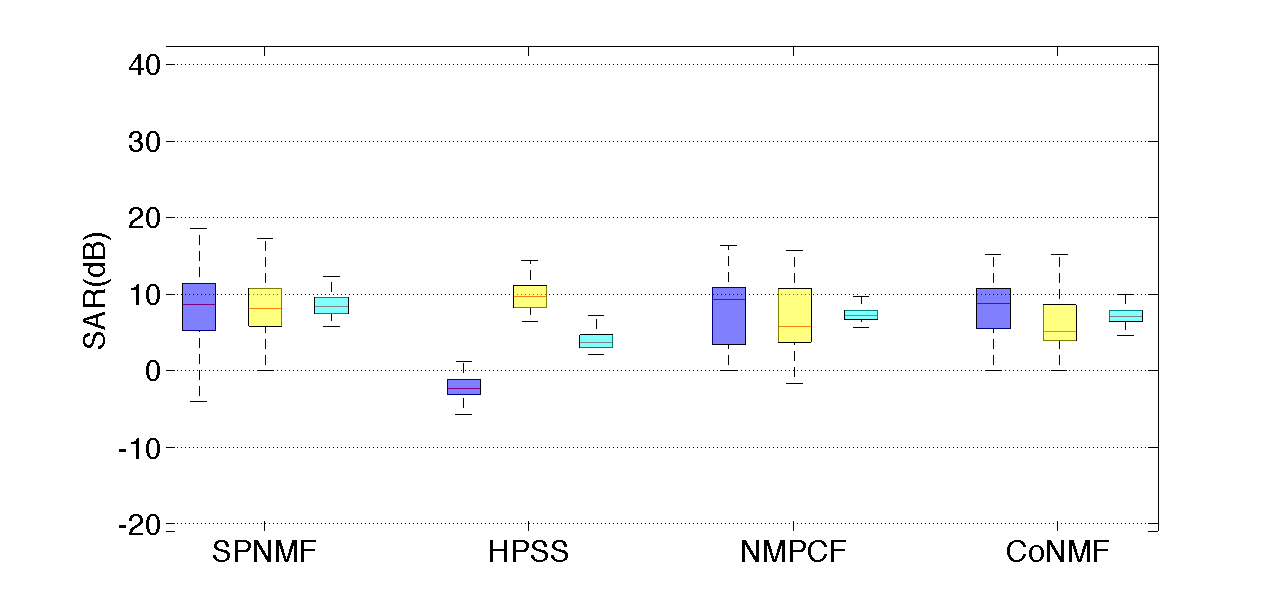
\includegraphics[width=9cm]{fig/DatabaseSAR.eps}
%  \vspace{2.0cm}
  \caption{\label{DatabaseSAR} SAR for percussive/left, harmonic/middle, mean/right separation results on the database for the four methods.}
  
\end{figure}




\subsection{Results on a genre specific database}
\label{sec:subdata}

The individual results on most of the songs of the database are similar to the average results. However, some interesting results were found on specific genres of music. Here we present the results obtained on the $14$ songs of the "Electronic/Fusion" music genre. These songs for the most part have a lot of silence and some solo parts played by only one instrument. Also, on some songs, the electronic drum repeats the same pattern during the whole song resulting in a very redundant drum part. The SDR results on the sub-database are displayed on Figure~\ref{ElectroFusionSDR} (the SIR and SAR results are represented in Appendix~\ref{appendix:sub_database} on Figures~\ref{ElectroFusionSIR} and~\ref{ElectroFusionSAR} respectively). 

The HPSS method gives competitive results, with a low variance for the percussive results and a good overall mean. The HPSS obtains consistent results throughout the database. The results on the genre specific database are significantly better than the ones on the whole database. It reflects the fact that the harmonic/percussive instruments are easier to separate on this genre of songs. 
 
The results of the NMPCF are the lowest of the four methods. The unconstrained harmonic part gives the NMPCF a higher degree of freedom which decreases the score as the information is unequally distributed in the harmonic and percussive layers depending on the signal to be decomposed. 

Finally the constrained NMF does not obtain satisfying results on this sub-database either. The hyper-parameters are set to the optimal values obtained on a training database of another genre. Because of that, the value of the parameters are not set correctly and similarly to the NMPCF, the information is not distributed in the appropriate harmonic/percussive parts. 


On this sub-database, the SPNMF clearly outperforms the other methods. Similarly to Section~\ref{subResults}, the percussive decomposition of the SPNMF has high variance because some of the instruments are not in the learning database. However, the mean of the percussive decomposition is significantly higher than the constrained NMF and the NMPCF. Furthermore, the harmonic decomposition and the mean results of the SPNMF are clearly above all the other methods. The SPNMF is effective to extract the redundant drum parts. Likewise, as the drum dictionary is fixed, it is unlikely for the percussive part to extract harmonic components. As the columns of $W_{H}$ are orthogonal, it is also unlikely for the harmonic part to extract percussive components. Contrary to the other algorithms, when the harmonic or percussive instruments are playing alone, the SPNMF does not extract any information in the percussive nor the harmonic part.



\begin{figure}[htb]

  \centering 
  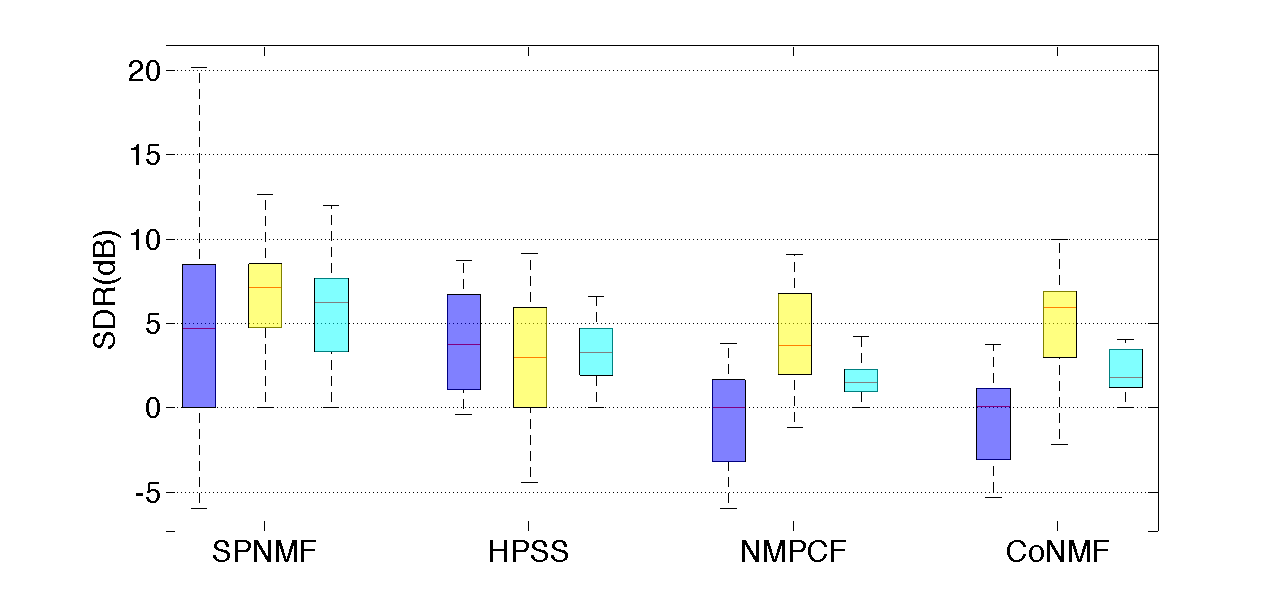
\includegraphics[width=9cm]{fig/ElectroFusionSDR.eps}
%  \vspace{2.0cm}
  \caption{\label{ElectroFusionSDR} SDR for percussive/left, harmonic/middle, mean/right separation results on the Electronic/Fusion songs for the four methods.}
  
\end{figure}

\subsection{Discussion}
\label{discu}

The results on the entire database give us insightful information.
The HPSS and the constrained NMF rely on the hypothesis that harmonic instruments have sparse tonal spectrogram and that percussive instruments have flat transient spectra. They utilize two different methods to extract the instruments the complementary median filtering, and constraints on the NMF decomposition.
The NMPCF uses prior learning to extract the percussive instruments in a specific part while the harmonic instruments are decomposed in an unconstrained layer. 
The SPNMF combines both techniques from the previous state of the art methods. It uses thus prior learning to extract the percussive instruments while the harmonic parts are extracted by the sparse PNMF components.



Each of the tested methods has its own advantages and  drawbacks. The HPSS is the easiest and the fastest method to implement and it does not require any hyper-parameter tuning. The results of the HPSS can be competitive when the harmonic instruments have smooth transients (i.e., sustained instruments such as the flute, the violin) and the percussive instruments have flat spectra (i.e., cymbal, snare drum). However, when the harmonic instruments have strong transients (glockenspiel, piano) and the percussive instruments have sparse spectra (bass drum, bongo) the HPSS does not give good results. 

The constrained NMF is based on the same hypothesis than the HPSS and has the same issue. Fine tuning of the hyper-parameters can alleviate the problem mentioned above but it is a tedious process and is not possible in the case of blind source separation. Our tests on a large database show that the constrained NMF is not robust enough for a wide variability of the analyzed signals.

Contrary to the results obtained in~\cite{canadas2014percussive} the NMPCF algorithm gives competitive results compare to the HPSS and the constrained NMF. However, as it uses training to guide the decomposition process, it requires a wide variety of information to perform on a large scale test. If the training database cannot contain sufficient information, the results will not be satisfying. 

On the large scale test, the SPNMF outperforms the other methods. It is able to extract the harmonic and the percussive instruments with higher score for the SDR, the SAR and the SIR. Using prior dictionary learning with a physical model on the harmonic instruments help to separate sources with much better accuracy.

In our test, the training database of the SPNMF and the NMPCF is only composed of drums sounds. The database~\cite{bittner2014medleydb} contains a wide variety of percussive instruments that are not in the training database. However, we decided not to include these types of percussion in the training database as we wanted to have a comparable computation time between the four methods and to test the robustness of the supervised methods when a percussive signal is not in the database. 


\section{Conclusion}
\label{sec:conc}

In this article, we demonstrate that SPNMF is a very promising model for harmonic/percussive decomposition. Indeed, the SPNMF outperforms three other state of the methods on the medley-dB database~\cite{bittner2014medleydb}. Carrying out an evaluation on a large database allowed us to compare more accurately the performance of the four methods on a large variety of music signals. 

%On a large database none of the state of the art methods produces a satisfying harmonic/percussive source separation. The large variety of audio signal makes the task extremely difficult. That said, on a smaller section of the database, the SPNMF showed some promising results (see~\ref{sec:subdata}).

We can say that the information from the drum dictionary built from the database ENST-Drums~\cite{gillet2006enst} is not sufficient to perform a harmonic/percussive source separation on a large scale. Depending of the style of music, some drums share similarities. A possible improvement would be to build genre specific drum dictionaries. In this way, the computation time would be reasonable as the amount information could be reduced and the templates of the dictionary could be a lot more focused on specific type of drums. 





\section*{Annexe}

\subsection{Euclidean distance}
\label{euclidisteq}

The euclidean distance gives us the problem,
$$\min_{W_1,W_2,H_2 \geq 0} \|V - W_{1}W_{1}^{T}V + W_{2} H_{2} \|^2.$$
The gradient wrt $W_1$ gives the update
$$[\nabla_{W_1} D(V|\tilde{V})]^{-} = 2 VV^TW_1, $$
and
\begin{align*}
[\nabla_{W_1} D(V|\tilde{V})]^{+} = 2VH_2^TW_2^TW_1 + W_2H_2V^TW_1 + \\ VV^TW_1W_1^TW_1 + W_1W_1^TVV^TW_1.
\end{align*}

Similarly, the gradient wrt $W_2$ gives
$$ [\nabla_{W_2} D(V|\tilde{V})]^{-} = VH_2^T $$
and
$$ [\nabla_{W_2} D(V|\tilde{V})]^{+} = 2W_1W_1^TVH_2^T + W_2H_2H_2^T.$$

Finally, the gradient wrt $H_2$ gives
$$ [\nabla_{H_2} D(V|\tilde{V})]^{-} = W_2^TV  $$
and
$$ [\nabla_{H_2} D(V|\tilde{V})]^{+} = 2W_2^TW_1W_1^TV + W_2^TW_2H_2. $$


\subsection{Kullback Leiber divergence}\label{KLdisteq}
The Kullback Leiber divergence gives us the problem,
$$\min_{W_1,W_2,H_2 \geq 0} V(log(V) - log(\tilde{V})) + (V-\tilde{V}).$$

The gradient wrt $W_1$ gives
$$[\nabla_{W_1} D(V|\tilde{V})]_{i,j}^{-} = (ZV^TW_1)_{i,j} + (VZ^TW_1)_{i,j},$$
with $Z_{i,j} = (\frac{V}{W_1W_1^TV + W_2H_2})_{i,j}$. The positive part of the gradient is
$$[\nabla_{W_1} D(V|\tilde{V})]^{+}_{i,j} = \sum_k(W^TV)_{j,k} + (\sum_{k}V_{i,k})(\sum_a W_{a,j}).$$


Similarly, the gradient wrt $W_2$ gives
$$ [\nabla_{W_2} D(V|\tilde{V})]^{-} = VH_2^T $$
and
$$ [\nabla_{W_2} D(V|\tilde{V})]^{+} = W_1W_1^TVH_2^T + W_2H_2H_2^T.$$

Finally, the gradient wrt $H_2$ gives
$$ [\nabla_{H_2} D(V|\tilde{V})]^{-} = W_2^TV  $$
and
$$ [\nabla_{H_2} D(V|\tilde{V})]^{+} = 2W_2^TW_1W_1^TV + W_2^TW_2H_2. $$

 
\subsection{Itakura Saito divergence}\label{ISdisteq}
The Itakura Saito divergence gives us the problem,
$$\min_{W_1,W_2,H_2 \geq 0} \frac{V}{\tilde{V}} - log(\frac{V}{\tilde{V}}) +1.$$

The gradient wrt $W_1$ gives
$$[\nabla_{W_1} D(V|\tilde{V})]_{i,j}^{-} = (ZV^TW_1)_{i,j} + (VZ^TW_1)_{i,j},$$
with $Z_{i,j} = (\frac{V}{W_1W_1^TV + W_2H_2})_{i,j}$. 
The positive part of the gradient is
$$[\nabla_{W_1} D(V|\tilde{V})]_{i,j}^{-} = (\phi V^TW_1)_{i,j} + (V \phi^T W_1)_{i,j},$$
with $$ \phi_{i,j} = (\frac{I}{W_1W_1^TV + W_2H_2})_{i,j}.$$ and $I = ones(size(V))$.


Similarly, the gradient wrt $W_2$ gives
$$ [\nabla_{W_2} D(V|\tilde{V})]^{-} = VH_2^T $$
and
$$ [\nabla_{W_2} D(V|\tilde{V})]^{+} = W_1W_1^TVH_2^T + W_2H_2H_2^T.$$

Finally, the gradient wrt $H_2$ gives
$$ [\nabla_{H_2} D(V|\tilde{V})]^{-} = W_2^TV  $$
and
$$ [\nabla_{H_2} D(V|\tilde{V})]^{+} = 2W_2^TW_1W_1^TV + W_2^TW_2H_2. $$



\subsection{SAR and SIR results with the different dictionaries}
\label{appendix:dict}

\begin{figure}[H]
  \centering 
  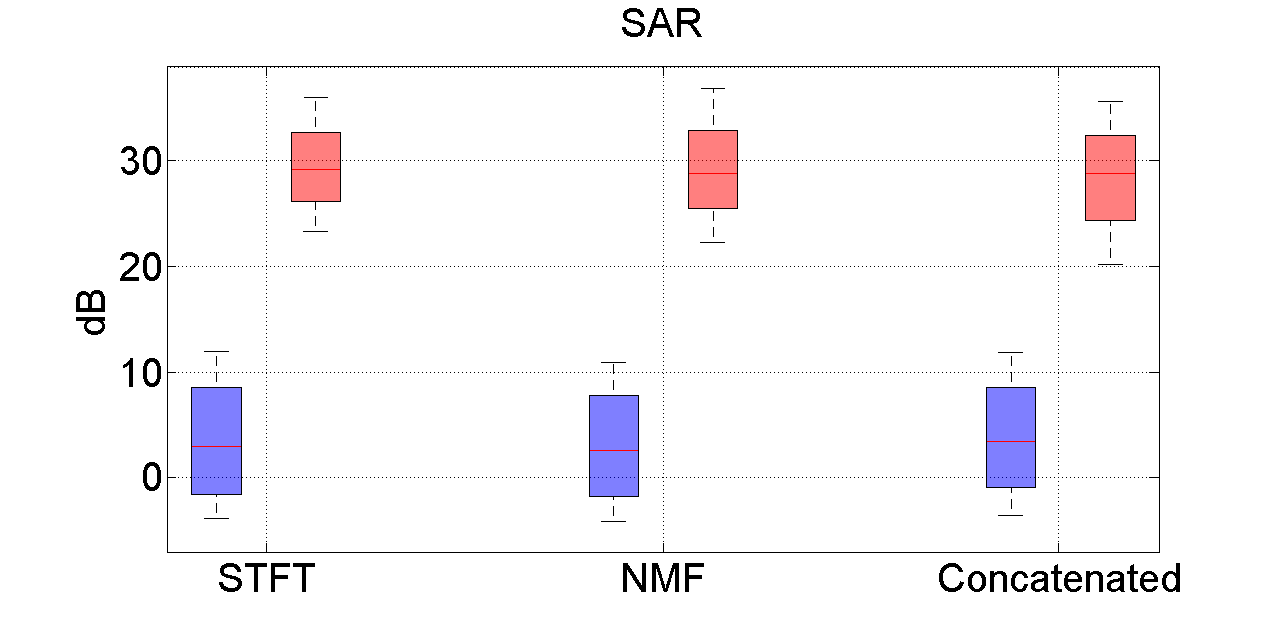
\includegraphics[width=8cm]{fig/DictSAR}
  \caption{\label{resultsDictSAR} SAR of harmonic (left bar)/percussive (right bar) estimated sources on the SiSec database with a STFT dictionary, a NMF dictionary and their concatenation.}
\end{figure}

\begin{figure}[H]
  \centering 
  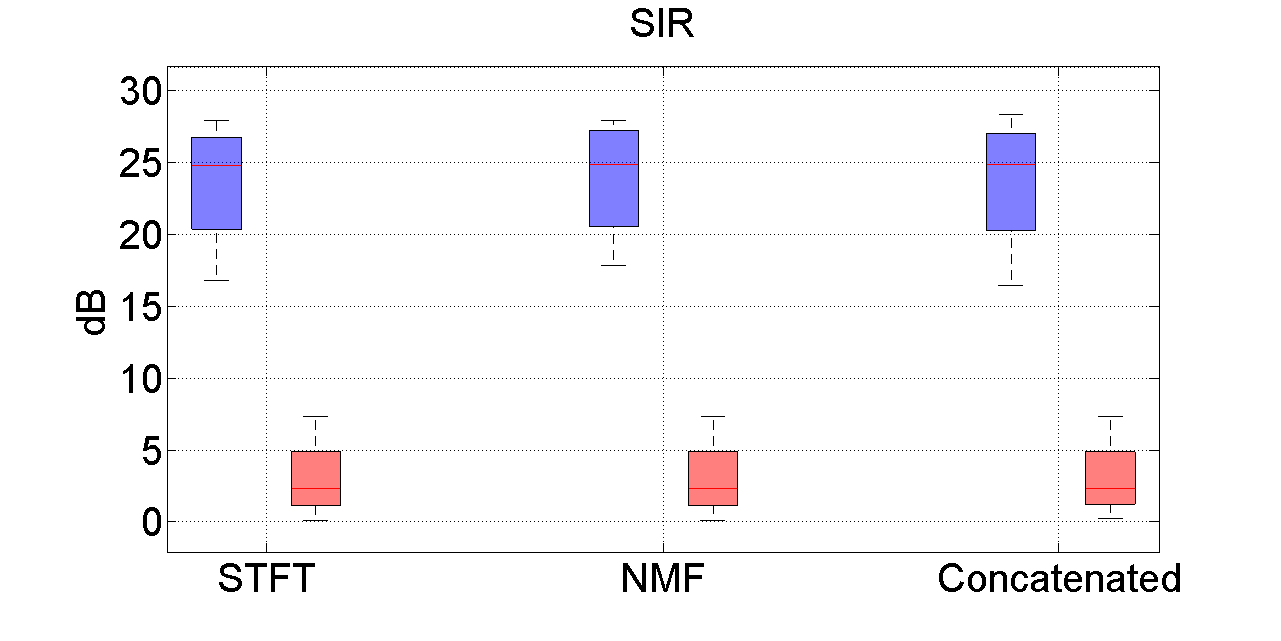
\includegraphics[width=8cm]{fig/DictSIR}
  \caption{\label{resultsDictSIR} SIR of harmonic (left bar)/percussive (right bar) estimated sources on the SiSec database with a STFT dictionary, a NMF dictionary and their concatenation.}
\end{figure}

\subsection{Results on the sub database}
\label{appendix:sub_database}

\begin{figure}[H]
  \centering 
  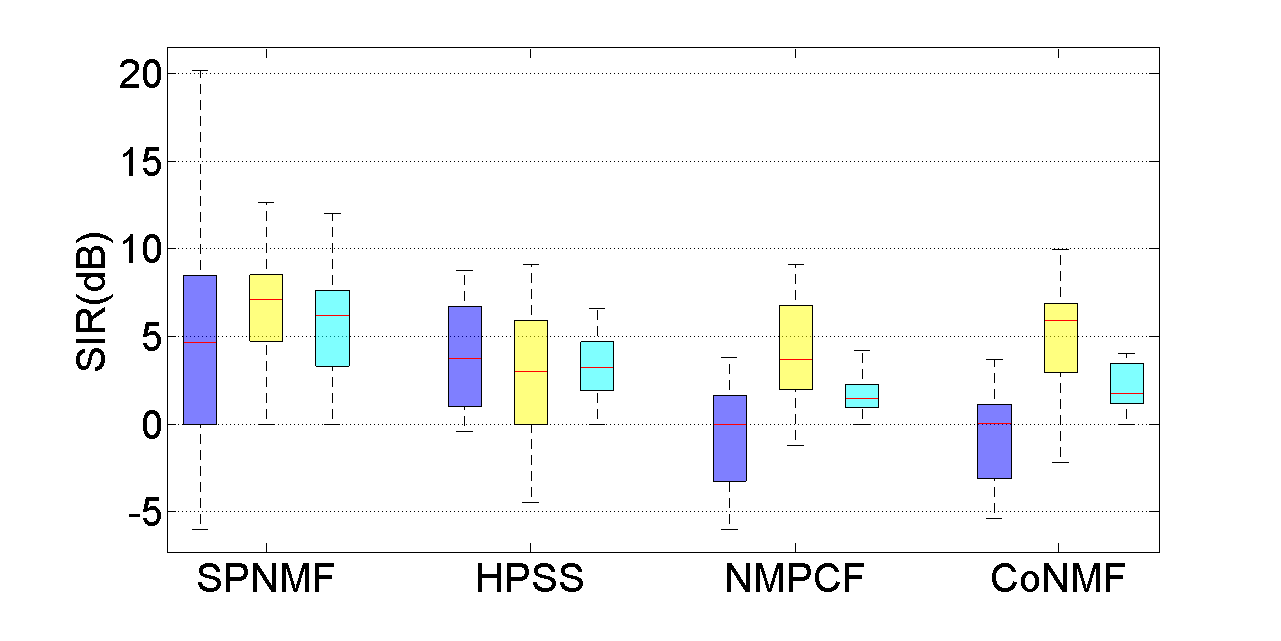
\includegraphics[width=9cm]{fig/ElectroFusionSIR}
  \caption{\label{ElectroFusionSIR} SIR for percussive/left, harmonic/middle, mean/right separation results on the Electronic/Fusion songs for the four methods.} 
\end{figure}

\begin{figure}[H]
  \centering 
  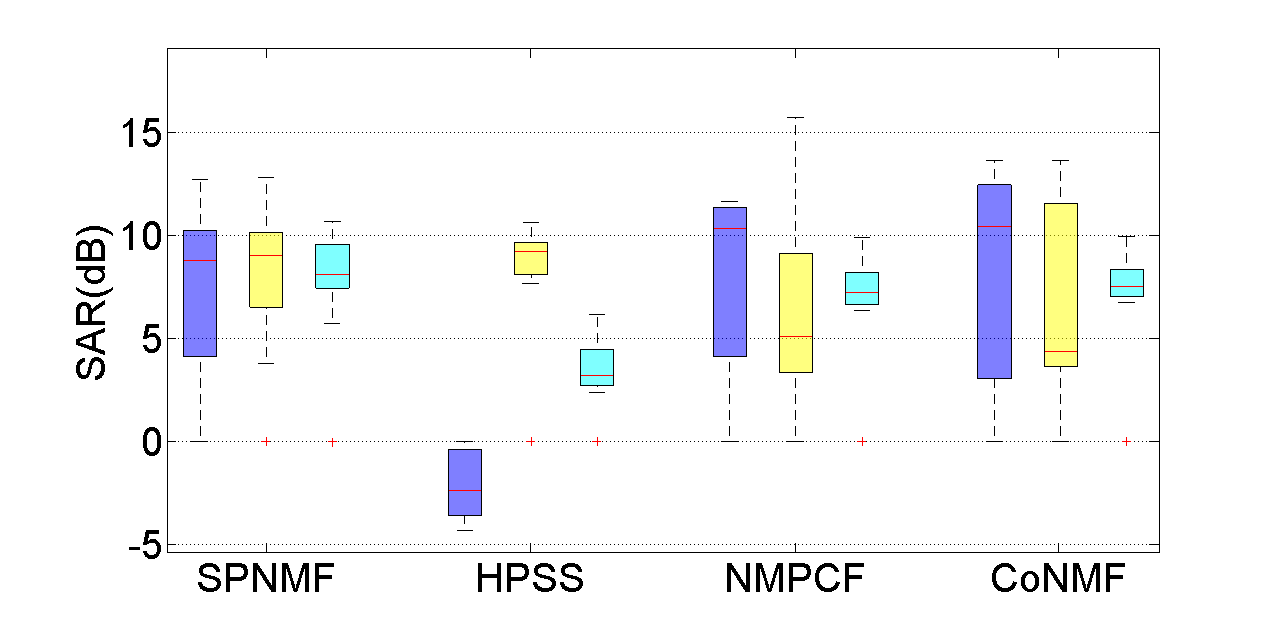
\includegraphics[width=9cm]{fig/ElectroFusionSAR}
  \caption{\label{ElectroFusionSAR} SAR for percussive/left, harmonic/middle, mean/right separation results on the Electronic/Fusion songs for the four methods.}
\end{figure}



\section*{Acknowledgment}




\bibliographystyle{IEEEtran}
% argument is your BibTeX string definitions and bibliography database(s)
\bibliography{reference}


\end{document}
